%start% Brought this in from Patrick thesis
\documentclass{thesis}
\usepackage[utf8]{inputenc}
\usepackage{parskip}
\usepackage{hepnames}
% \usepackage[printonlyused]{acronym}
\usepackage{thesis}
\usepackage{ptdr-definitions}
\usepackage{hepnicenames}
\usepackage{hepunits}
\usepackage{abhep}
\usepackage{slashed}
\usepackage{multirow}
%end%
%\documentclass[hyperpdf]{hepthesis}
%\documentclass[a4paper,10pt]{book}
%\usepackage{fullpage}
%\usepackage[margin=2cm]{geometry} % Defining geometry of the usable text space

%% Using Babel allows other languages to be used and mixed-in easily
%\usepackage[ngerman,english]{babel}
% \usepackage[english]{babel}
% \selectlanguage{english}

%% Citation system tweaks
% \usepackage{cite}

% \usepackage{amsmath}
% \usepackage{amsthm}
% \usepackage{amsfonts}
% \usepackage{amssymb}
% \usepackage{graphicx}
% \usepackage{color}                 % For color (highlights,...) 
% \usepackage{caption}               % ?????
% \usepackage{soul}                  % For text highlights
% \usepackage{threeparttable}        % Better tables

% \usepackage{hyperref}              % Need after glossaries (allows links)
\usepackage[toc,acronym]{glossaries} %(recommended) for the indexing phase, as opposed to makeindex (the default)
\makeglossaries
% \newacronym[longplural={Frames per Second}]{fpsLabel}{FPS}{Frame per Second}

%A
\newacronym{ALICE}{ALICE}{A Large Ion Collider Experiment}
\newacronym{ATLAS}{ATLAS}{A Toroidal LHC ApparatuS}
\newacronym{APD}  {APD}  {Avalanche photo-diodes}

%B
\newacronym{BSM}{BSM}{Beyond the Standard Model}
\newacronym{BDT}{BDT}{Boosted Decision Tree}

%C
\newacronym{CERN}{CERN}{European Organization for Nuclear Research} %derived from the name Conseil Européen pour la Recherche Nucléaire
\newacronym{CMS} {CMS} {Compact Muon Solenoid}

%D
\newacronym{DAQ}{DAQ}{Data Acquisition}
\newacronym{DQM}{DQM}{Data Quality Monitoring}

%E
\newacronym{EB}  {EB}  {ECAL Barrel}
\newacronym{EE}  {EE}  {ECAL Endcap}
\newacronym{ECAL}{ECAL}{Electromagnetic Calorimeter}

%F
\newacronym{FCT}{FCT}   {Fundação para a Ciência e a Tecnologia}

%G

%H
\newacronym{HCAL}{HCAL}  {Hadronic Calorimeter}
\newacronym{HLT} {HLT}   {High Level Trigger}

%I

%J
\newacronym{JER}{JER}{jet energy resolution}
\newacronym{JES}{JES}{jet energy scale}

%K

%L
\newacronym{L1T}   {L1T}   {Level 1 Trigger}
\newacronym{LINAC2}{LINAC2}{Linear Particle Accelerator 2}
\newacronym{LHC}   {LHC}   {Large Hadron Collider}

%M
\newacronym{MC} {MC} {Monte Carlo}
\newacronym{MET}{MET}{Missing Transverse Energy}

%N

%O

%P
\newacronym{PS} {PS} {Proton Synchrotron}
\newacronym{PSB}{PSB}{Proton Synchrotron Booster}

%Q

%R

%S
\newacronym{SM} {SM} {Standard Model}
\newacronym{SPS}{SPS}{Super  Proton Synchrotron}

%T

%U

%V
\newacronym{VBF}{VBF}{vector Boson Fusion}
\newacronym{VPT}{VPT}{Vacuum Photo-Triodes}
%W

%X

%Y

%Z


% \acro{CL}{confidence level}
% \acro{CSC}{cathode strip chamber}
% \acro{CSV}{combined secondary vertex}
% \acro{CTF}{combinatorial track finder}
% \acro{DA}{deterministic annealing}
% \acro{DT}{drift tube}
% \acro{GSF}{Gaussian sum filter}
% \acro{HB}{hadron barrel}
% \acro{HE}{hadron endcaps}
% \acro{HF}{hadron forward}
% \acro{HLT}{high-level trigger}
% \acro{HO}{hadron outer}
% \acro{HPS}{hadron plus strips}
% \acro{JER}{jet energy resolution}
% \acro{JES}{jet energy scale}
% \acro{L1}{Level-1}
% \acro{LHCHXSWG}{LHC Higgs Cross Section Working Group}
% \acro{LO}{leading order}
% \acro{MPF}{missing transverse energy projection fraction}
% \acro{MPI}{multi-parton interaction}
% \acro{MVA}{multi-variate analysis}
% \acro{MSSM}{minimal supersymmetric standard model}
% \acro{NLO}{next-to-leading order}
% \acro{NNLO}{next-to-next-to-leading order}
% \acro{NNLL}{next-to-next-to-leading logarithmic}
% \acro{pdf}{probability density function}
% \acro{PDF}{parton distribution function}
% \acro{PF}{particle flow}
% \acro{PS}{Proton Synchrotron}
% \acro{PSB}{Proton Synchrotron Booster}
% \acro{PU}{pile-up}
% \acro{PV}{Primary Vertex}
% \acro{QCD}{Quantum Chromodynamics}
% \acro{RF}{radio frequency}
% \acro{RPC}{resistive plate chamber}
% \acro{SPS}{Super Proton Synchrotron}
% \acro{SSV}{simple secondary vertex}
% \acro{SM}{standard model}
% \acro{TEC}{tracker endcaps}
% \acro{TIB}{tracker inner barrel}
% \acro{TID}{tracker inner disks}
% \acro{TOB}{tracker outer barrel}
% \acro{UE}{underlying event}
% \acro{VBF}{vector boson fusion}
% \acro{WLCG}{Worldwide LHC Computing Grid}


\title{Search for Higgs Decay to Dark Matter and Trigger Studies} 
\author{João Carlos Arnauth Pela}
% \email[Contact email: ]{joaopela@gmail.com}
% \affiliation{Imperial College London}
% \keywords{Particle Physics}
\date{21 September 2015}


%% Doc-specific PDF metadata
\makeatletter
\@ifpackageloaded{hyperref}{
\hypersetup{
  pdftitle    = {Search for Higgs Decay to Dark Matter and Trigger Studies},
  pdfsubject  = {João Pela's PhD thesis},
  pdfkeywords = {LHC, CMS, Higgs, Dark Matter, Trigger},
  pdfauthor   = {\textcopyright\ João Pela}
}
}{}
\makeatother

\begin{document}

\begin{frontmatter}
  %% Title
%!!UPDATE THIS
\titlepage[of Imperial College London]%
{A dissertation submitted to Imperial College London\\
  for the degree of Doctor of Philosophy}
  
\clearpage
\textbf{The copyright of this thesis rests with the author and is made available under a Creative Commons 
Attribution Non-Commercial No Derivatives licence. Researchers are free to copy, distribute or 
transmit the thesis on the condition that they attribute it, that they do not use it for commercial 
purposes and that they do not alter, transform or build upon it. For any reuse or redistribution, 
researchers must make clear to others the licence terms of this work.}


%% Abstract
\begin{abstract}%[\smaller \thetitle\\ \vspace*{1cm} \smaller {\theauthor}]
The Compact Muon Solenoid (CMS) is a general-purpose particle detector at the CERN Large Hadron Collider (LHC). The goal of this experiment is to search for the Higgs boson and evidence of new physics and to test the prediction of the Standard Model (SM) at the TeV scale. This thesis describes the analysis of proton-proton collision data recorded by CMS during 2012 and support work for data taking during the same period.

A search for the Vector Boson Fusion (VBF) produced Higgs boson invisible decays, using $19.5\,\femto\barn^-1$ of data recorded with prompt reconstruction triggers at a center of mass energy of $8\,\TeV$, is presented. Events are selected with two forward jets and large Missing Transverse Momentum. Assuming the SM VBF production cross section and acceptance, the observed (expected) upper limit at the 95\% confidence level on the \BRinv\, is determined to be of 65\% (49\%) for $m_H=125\,\GeV$.

A second search for the VBF Higgs boson invisible decays, using $19.2\,\femto\barn^-1$ of data recorded with delayed reconstruction (parked) triggers at a center of mass energy of $8\,\TeV$, is also presented. A new event selection criteria was developed taking advantage of the lower trigger requirements. Assuming the SM VBF Higgs production cross section and acceptance, the observed (expected) upper limit at the 95\% confidence level on the \BRinv\, is determined to be of 57\% (40\%) for $m_H=125\,\GeV$.

Monitoring for the CMS Level 1 Trigger system has been developed and used during the 2012 and subsequent LHC data acquisition periods. Contribution to the high reliability of this system during data taking and providing crucial information for validation of the data quality.
\end{abstract}

%DONE

%% Declaration
\begin{declaration}
I declare that the work contained in this thesis is my own, and all results and figures taken from other sources are indicated in the text and referenced appropriately. The analyses presented in this thesis were developed in close collaboration with other members of the CMS experiment.

For the Vector Boson Fusion (VBF) Higgs to invisible prompt analysis I have contributed with the literature review and final background cross section input values for background normalization. QCD multi-jet background studies were also preformed with the target of improving the final selection or prepare the parked analysis, this analysis is presented to give context for the more important work developed later. 

For the VBF Higgs to invisible parked analysis I have participated in the development of the parked trigger, which was used to record the majority of the analysed data. I have continued the QCD multi-jet background studies which have lead to the production of dedicated Monte Carlo simulations and novel approaches to reject this type of events. I have been the responsible for the cross check analysis of the main result which has successfully validated the implementation of the main analysis \cite{ARTICLE:CMSVBFHiggsInvisibleParkedAnalysisPAS}. It is a normal a requirement for many \gls{CMS} publications to have a cross check analysis implemented independently from the main result in order to be able to ensure the accuracy of the final results. I have also participated in the preparation of the Run II analysis where I have lead the development of both the triggers used for data recording during 2015. Additionally, I have developed a method to create the first QCD multi-jet Monte Carlo sample with no MET requirements with signal like properties.

As part of the CMS Level 1 Trigger (L1T) Detector Performance Group (DPG) I have developed monitoring tools for this system, which were both used for real-time monitoring and posterior data certification for physics analysis usage. My work in this group has lead to my appointment for two years to the position of coordinator of the \gls{CMS} \gls{L1T} Data quality Monitoring software development team. Field work was also performed by doing shifts as Trigger and Shift Leader in the experiment control room and on call shifts as the Trigger Detector on Call (DOC) expert.
 
\vspace*{1cm}
\begin{flushright}
João Pela
\end{flushright}
\end{declaration}

%% Acknowledgements
\begin{acknowledgements}
I would like to thank the Imperial College HEP Group and the FCT for supporting and giving me the opportunity to pursue research including my time spent at CERN. Thanks to my supervisor, David Colling, for his guidance during the years of my PhD, the many useful discussions and his enthusiasm for particle physics research. Thanks must also go to all my colleagues of the CMS VBF Higgs to invisible group with whom I have worked directly, Patrick Dunne, Anne-Marie Magnan, Alexandre Nikitenko, Jim Brooke and Chayanit Asawatangtrakuldee. Thanks to everyone in CMS L1T DPG group, specially to Carlo Battilana and Arno Heister for their support. Thanks to all my friends that supported me on my way to finish this degree, it is difficult to mention all of you, but here is a small list, Antonio Pacheco, André David, Alice Mitchell, Chris Holdsworth-Swan, Francisco Sousa, Glenn Spiers, Guillermo Marrero, João Filipe, Miguel Cunhal, Miguel Machado, Nadia Silva, Raquel Monteiro, and many, many more. Finally, and most importantly, I thank my parents and grandparents for their constant support, love and encouragement.
\end{acknowledgements}

\clearpage

\vspace*{\fill}
The work presented in this thesis was supported by the Portuguese Government through \gls{FCT} in the form of my PhD grant with the reference SFRH/BD/77979/2011. I am thankful for their support which allowed me to attain higher education.
\vspace*{\fill}

\begin{center}
\resizebox{1.0\linewidth}{!}{

\includegraphics{FrontMatter/Images/FundingBand.png}
}
\end{center}


% \begin{preface}
% Thesis structure and so on...
% \end{preface}

\dedication{To my grandmother.}

%% Preface
%\begin{preface}
%\end{preface}

%% ToC
\tableofcontents

\newpage
\listoffigures

\newpage
\listoftables

%% Strictly optional!
%\frontquote%
%{Writing in English is the most ingenious torture\\
%   ever devised for sins committed in previous lives.}%
%  {James Joyce}
 
% \titlepage[of the High Energy Physics Group]{%
%   A dissertation submitted to the Imperial College London\\ for the degree of Doctor of Philosophy}

\end{frontmatter}

\begin{mainmatter}
  \chapter{Theory}
%NOTE: Maybe would be good to make a more descriptive title

\colorbox{red}{
\begin{minipage}{0.95\linewidth}
TODO: 
\begin{itemize}
  \item Global status
\end{itemize}

\end{minipage}
}

\section{Standard Model of Particle Physics}

\colorbox{red}{
\begin{minipage}{0.95\linewidth}
TODO: 

\begin{itemize}
  \item Very brief summary of the Standard Model.
\end{itemize}

\end{minipage}
}

The \gls{SM} of particle physics is the currently accepted model for describing the physics of elementary particles.

\begin{table}[!htb]
  \centering
  \begin{tabular}{|c|c|c|c|c|}
  \hline
  \multicolumn{5}{|c|}{Leptons (J=1/2)} \\
  \hline
  Generation & Particle Name & Symbol & Mass ($GeV/c^2$) & Q/e \\
  \hline
  \hline
  \multirow{2}{*}{$1^{st}$} & Electron          & e          &           0.000511    & 1 \\
                            & Electron Neutrino & $\nu_e$    & $< 3 \times 10^-9$    & 0 \\
  \hline
  \hline
  \multirow{2}{*}{$2^{nd}$} & Muon              & $\mu$      &              0.106    & 1 \\
                            & Muon Neutrino     & $\nu_\mu$  & $< 1.9 \times 10^-4$  & 0 \\
  \hline
  \hline
  \multirow{2}{*}{$3^{rd}$} & Tau               & $\tau$     & 1.777                 & 1 \\
                            & Tau Neutrino      & $\nu_\tau$ & $< 1.82 \times 10^-2$ & 0 \\
  \hline
  \end{tabular}
  \caption[List of leptons and their fundamental properties]{List of leptons and their fundamental properties}
  \label{TheoreticalIntroduction_LeptonProperties}
\end{table}

\begin{table}[!htb]
  \centering
  \begin{tabular}{|c|c|c|c|c|}
  \hline
  \multicolumn{5}{|c|}{Quarks (J=1/2)} \\
  \hline
  Generation & Particle Name & Symbol & Mass ($GeV/c^2$) & Q/e \\
  \hline
  \hline
  \multirow{2}{*}{$1^{st}$} & Up      & u & $1.5-3.3 \times 10^{-3}$ & -2/3 \\
                            & Down    & d &   $3.5-6 \times 10^{-3}$ &  1/3 \\
  \hline
  \hline
  \multirow{2}{*}{$2^{nd}$} & Charm   & c &                1.16-1.34 & -2/3 \\
                            & Strange & s &  $70-130 \times 10^{-3}$ &  1/3 \\
  \hline
  \hline
  \multirow{2}{*}{$3^{rd}$} & Top     & t &                  169-173 & -2/3 \\
                            & Bottom  & b &              $4.13-4.37$ &  1/3 \\
  \hline
  \end{tabular}
  \caption[List of quarks and their fundamental properties]{List of quarks and their fundamental properties}
  \label{TheoreticalIntroduction_QuarkProperties}
\end{table}

\begin{table}[!htb]
  \centering
  \begin{tabular}{|c|c|c|c|c|}
  \hline
  \multicolumn{4}{|c|}{Bosons} \\
  \hline
   Particle Name & Mass ($GeV$) &     Q/e & Spin \\
  \hline
  \hline
  Photon ($\gamma$) &                  0 &       0 &    1 \\
  \hline
  $W^\pm$           & $80.385 \pm 0.015$ & $\mp 1$ &    1 \\
  $Z^0$             & $91.1876\pm0.0021$ &       0 &    1 \\
  \hline
  Gloun (g)         &                  0 &       0 &    1 \\
  \hline
  \end{tabular}
  \caption[List of bosons and their fundamental properties]{List of force carrying bosons and their fundamental properties \cite{ARTICLE:PDG2014}.}
  \label{TABLE:Theory_SM_ParticlesAndForces_BosonProperties}
\end{table}


\section{Higgs Mechanism}

Summary of the Higgs Mechanism. Should include
\begin{itemize}
 \item Motivations 
 \item Explanation of the mechanism itself
 \item Consequences 
 \item Possible decays
\end{itemize}

\section{Higgs Invisible decays}

\colorbox{red}{
\begin{minipage}{0.95\linewidth}
TODO: 
\begin{itemize}
  \item Explain what are SM Higgs invisible decays.
  \item Go over the possibility of BSM invisible decays.
\end{itemize}

\end{minipage}
}


  \chapter{Experimental Apparatus}
\label{CHAPTER:ExperimentalApparatus}

\glsresetall % Resetting all acronyms

%%%%%%%%%%%%%%%%%%%%%%%%%%%%%%%%%%%%%%%%%%%%%%%%%%%%%%%%%%%%%%%%%%%%%%%%%%%%%%%%%%%%%%%
%%% SECTION
%%%%%%%%%%%%%%%%%%%%%%%%%%%%%%%%%%%%%%%%%%%%%%%%%%%%%%%%%%%%%%%%%%%%%%%%%%%%%%%%%%%%%%%
\section{The Large Hadron Collider}
\label{SECTION:ExperimentalApparatus_LHC}

% Status: DONE (reviewed J.Pela x1)
%
% TODO:
% * DONE: LHC location, size, particles used, energy usage.
% * Basics of machine and operation
% * How instantaneous luminosity is calculated include Instantaneous luminosity equation
% * Delivered instantaneous luminosity Run I (proton-Proton)

% \colorbox{red}{
% \begin{minipage}{0.95\linewidth}
%  
% \begin{itemize}\item\end{itemize}
% \end{minipage}
%}

% CERN and LHC Location
The \gls{LHC} \cite{ARTICLE:LHCDesignReportVol1,ARTICLE:LHCMachine} is currently the world's largest particle accelerator and is capable of producing the highest energy particle beams ever made by mankind. This machine has total perimeter of $26.7\,\kilo\meter$ and was built at \gls{CERN} in a circular tunnel, which previously housed the \gls{LEP} \cite{LEPTDR:LEPInjectorStudyGroup}, at an average depth of $100\,\meter$ below ground under the Franco-Swiss border near Geneva, Switzerland. A diagram of the \gls{LHC} tunnel and its experiments can be found at figure \ref{FIGURE:ExperimentalApparatus_LHCLayoutUnderground}.

\begin{figure}[!htb]
  \centering
  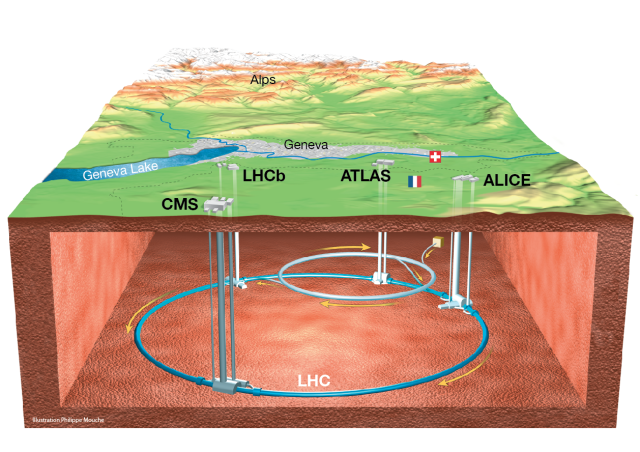
\includegraphics[width=0.70\textwidth]{Chapter02/LHC/Images/LHCUnderGroundDiagram.png}
  \caption{Underground diagram of the Geneva area showing the \gls{LHC} and its experiments location \cite{IMAGEREF:LHCDiagram}.}
  \label{FIGURE:ExperimentalApparatus_LHCLayoutUnderground}
\end{figure}

% Structure and experiments
The \gls{LHC} is a synchrotron machine with the capability of accelerating two particles beams in opposite directions in two separated beam pipes. These beams only cross and are forced to collide in four points of the accelerator where particle detectors are installed to observe the products of such collisions. This experiments are: \gls{ATLAS} \cite{ARTICLE:TheATLASExperiment}, \gls{CMS} \cite{ARTICLE:TheCMSExperiment}, \gls{LHCb} \cite{ARTICLE:TheLHCbExperiment} and \gls{ALICE} \cite{ARTICLE:TheALICEExperiment}.
% Add other experiments?

% Objective
The objective of the \gls{LHC} program is to investigate physics at the $\TeV$ scale, more specifically to understand the electroweak symmetry breaking and if this phenomena could be explained by the Higgs mechanism. There are many \gls{BSM} models that predict new physics at this energy regime making the \gls{LHC} the perfect machine to investigate such phenomena. \gls{ATLAS} and \gls{CMS} are general-purpose detectors which aim to investigate a broad spectrum of physics. The \gls{LHCb} detector is used to study processes that involve the decay of b-flavoured hadrons. The \gls{ALICE} detector is optimised to look at heavy-ion collisions and to investigate the properties of extreme high density medium that is formed.

% CERN accelerator chain
The \gls{LHC} is only the last element of a complex accelerator chain which step-by-step increases the energy of the particles to eventually be collided \cite{ARTICLE:LHCMachine}. Protons are initially obtained by stripping the electrons of hydrogen gas. This process happens at the begging of the \gls{LINAC2} which then accelerates them up to the energy of $50\,\MeV$. After this initial step proton are injected into the \gls{PSB} and the energy ramps ups to $1.4\,\GeV$. Particles are then passed to the \gls{PS} where the energy futher increases to $25\,\GeV$. Subsequently they are the injected into the \gls{SPS} where the particle energy level reaches $450\,\GeV$. Finally, protons pass to the \gls{LHC} where they can be accelerated to a maximum energy of $7\,\TeV$. A simplified diagram of the \gls{CERN} accelerator chain can be found in figure \ref{FIGURE:ExperimentalApparatus_LHCAccelaratorChain}. 
Normal operation of the \gls{LHC} therefore depends on all the upstream accelerators availability. The typically turn around time, the time necessary to stop the accelerator from running and restart collisions, is around 2 hours. When stable beams are achieved, a single proton fill can be used to collide protons up to 24 hours, but it is common to restart more frequently to profit from the higher collision rates possible right at the beginning of a new fill.

\begin{figure}[!htb]
  \centering
  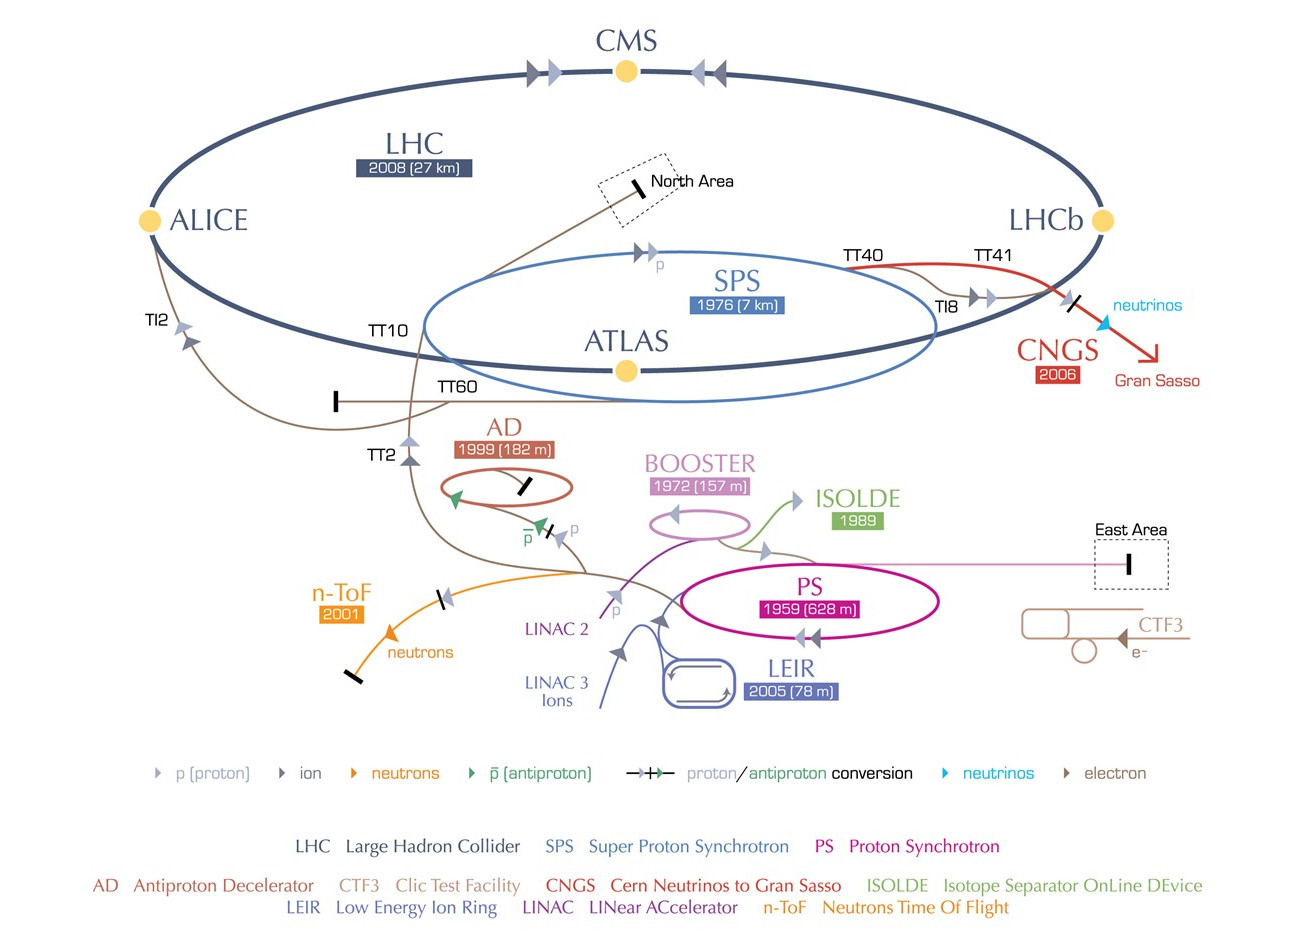
\includegraphics[width=0.90\textwidth]{Chapter02/LHC/Images/CERNAcceleratorComplex.jpg}
  \caption{Diagram of the \gls{CERN} accelerator complex \cite{IMAGEREF:CERNAcceleratorComplex}.}
  \label{FIGURE:ExperimentalApparatus_LHCAccelaratorChain}
\end{figure}

% LHC modes of opperation
Each beam pipe can be filled with proton or heavy ions. Three modes of operation have been tried: proton-proton, proton-lead ion and lead ion-lead ion. By changing the incoming particles we are changing the quantity of nucleons present at each interaction. The maximum design energy per proton is $7\,\TeV$ and is $2.76\,\TeV$ for each lead nucleon. The maximum design luminosity for proton-proton is $10^{34}\,\cm^{-2}\second^{-1}$ and $10^{27}\,\cm^{-2}\second^{-1}$ for lead ion-lead ion collisions.

% LHC structure
Particles beams trajectory are curved by 1232 niobium-titanium superconducting dipole magnets each with a length of $14.3\,\meter$. They are cooled with superfluid helium to $1.9\,\kelvin$ and produce the necessay magnetic field of $8.4\,\tesla$. Eight \gls{RF} cavities located at the \gls{LHC} point 4 are used to accelerate the beams. At each turn particle energy is increased to compensate for synchrotron radiation loss and increase the momentum. At nominal operation the \gls{LHC} will steer 2808 bunches composed up to $10^{11}$ protons separated by $25\,\ns$ in each direction. Some of the key parameters of the \gls{LHC} proton-proton and lead-lead operation can be found in table \ref{TABLE:ExperimentalApparatus_LHCMachineParameters}.

\begin{table}[!htb]
  \centering
  \begin{threeparttable}
    \begin{tabular}{|lcccc|}
    \hline 
                                  &              &           \textit{pp} &         \textbf{HI} &  \\
    \hline\hline
    Energy per nucleon            & E            &                     7 &                2.76 &                 $\TeV$ \\
    Dipole field at 7 TeV         & \textit{B}   &                  8.33 &                8.33 &               $\tesla$ \\
    Design Luminosity\tnote{*}    & $\mathcal{L}$ &            $10^{34}$ &           $10^{27}$ & $\cm^{-2}\second^{-1}$ \\
    Bunch separation              &              &                    25 &                 100 &                  $\ns$ \\
    No. of bunches                & $k_B$        &                  2808 &                 592 &                        \\
    No. particles per bunch       & $N_p$        & $1.15 \times 10^{11}$ & $7.0 \times 10^{7}$ &                        \\
    \hline
    \hline
    \textbf{Collisions}           &              &  &  &  \\
    \hline
    $\beta$-value at IP           & $\beta^{*}$  &                  0.55 &                 0.5 &        $\meter$ \\
    RMS beam radius at IP         & $\sigma^{*}$ &                  16.7 &                15.9 &  $\micro\meter$ \\
    Luminosity lifetime           & $\tau_L$     &                    15 &                   6 &         $\hour$ \\
    Number of collisions/crossing & $n_c$        &          $\approx 20$ &                   - &                 \\
    \hline
    \end{tabular}
    \begin{tablenotes}
      \item[*] For heavy-ion (HI) operation the design luminosity for Pb-Pb collisions is given.
    \end{tablenotes}
  \end{threeparttable}
  \caption[LHC parameters relevant for detectors]{The machine parameters relevant for the 
                                                  LHC detectors.\cite{CMSTDR:CMSPhysicsVol1}}
  \label{TABLE:ExperimentalApparatus_LHCMachineParameters}
\end{table}


At the \gls{LHC} we are looking for extremely rare processes. As is can be seen in figure \ref{FIGURE:ExperimentalApparatus_LHCCrossSections} the production cross section of a \gls{SM} Higgs boson is more than 9 orders of magnitude smaller than the total proton-proton cross section. 

\begin{figure}[!htb]
  \centering
  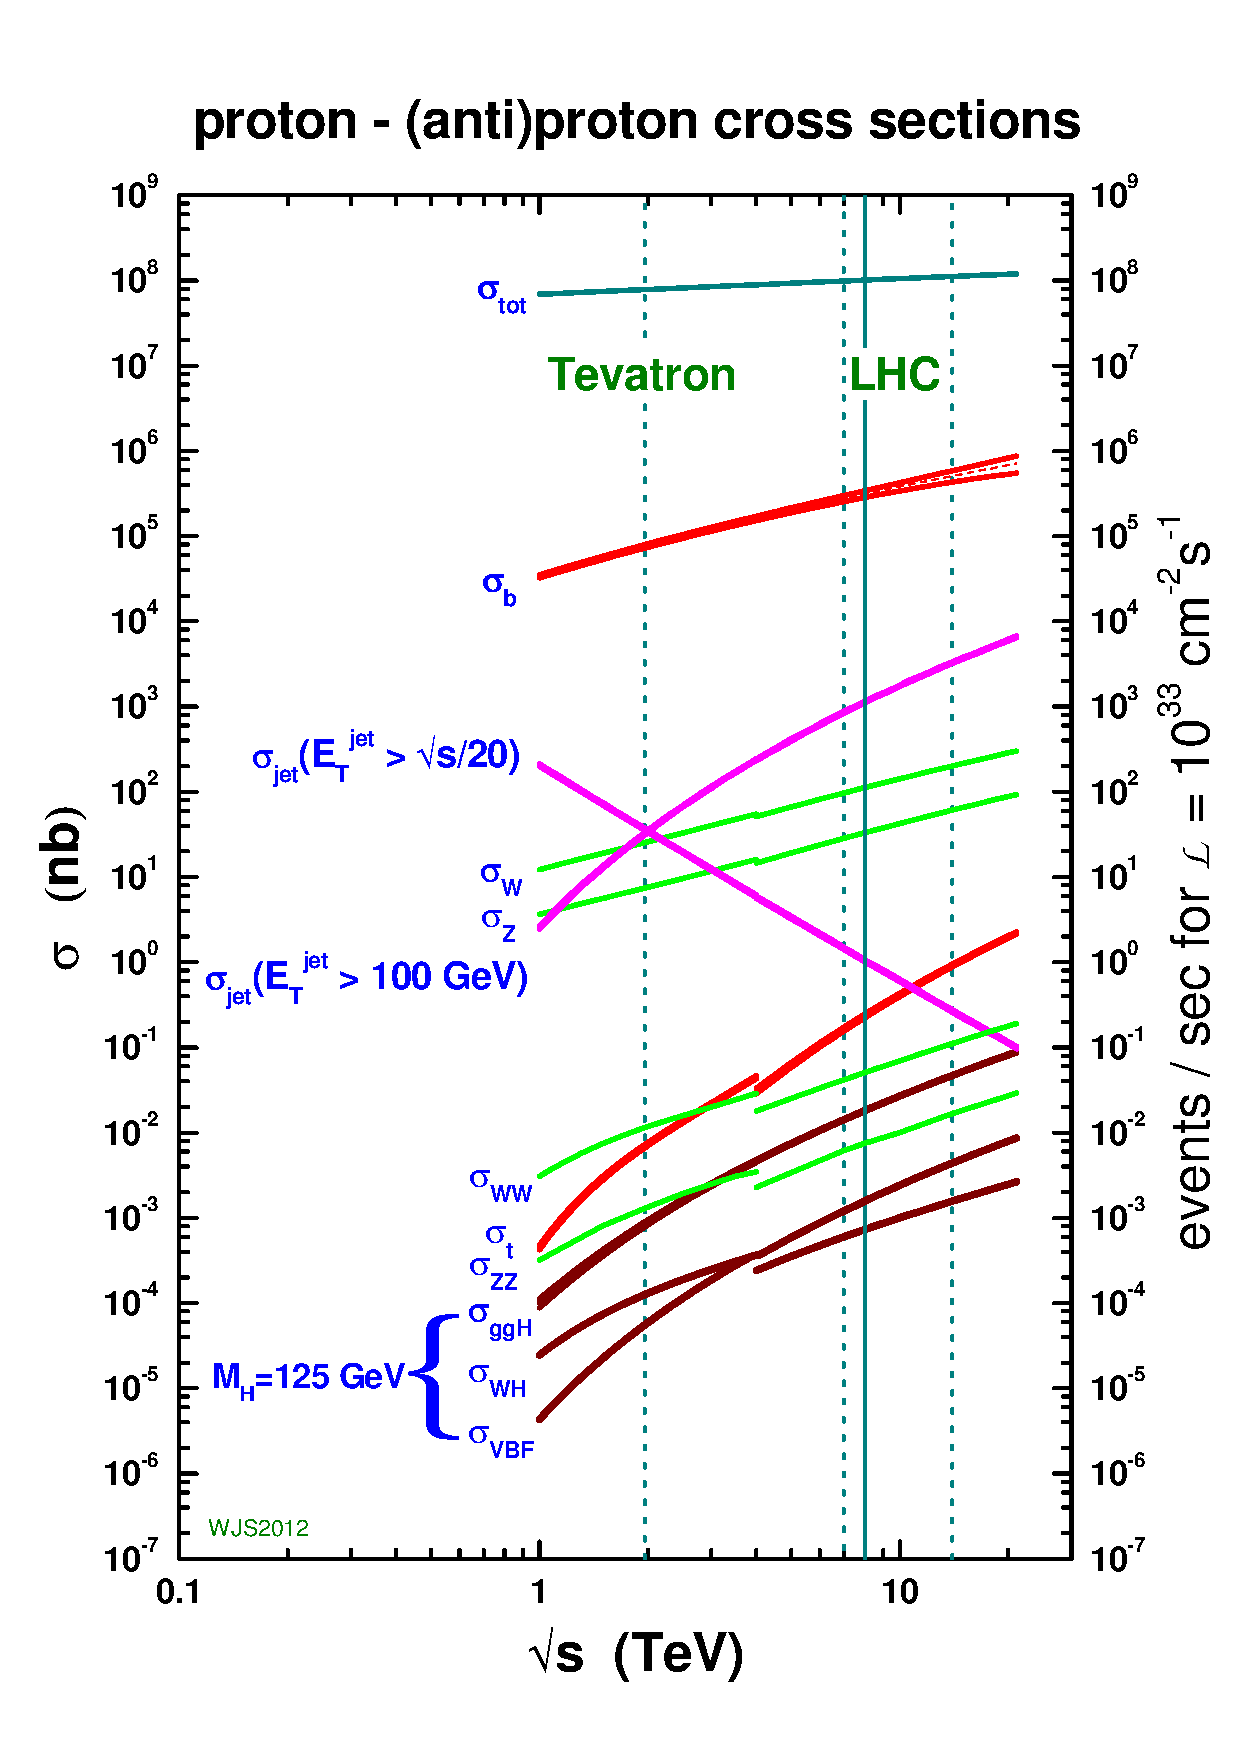
\includegraphics[width=0.50\textwidth]{Chapter02/LHC/Images/crosssections2012_v5}
  \caption{Cross sections for several processes for collisions of antiproton-proton and proton-proton as a function of the center of mass energy \cite{ARTICLE:TheCMSExperiment}.}
  \label{FIGURE:ExperimentalApparatus_LHCCrossSections}
\end{figure}

To be able to record and study such rare processes we need to produce a significant number of collisions. For this purpose the \gls{LHC} was designed to operate at high instantaneous luminosity, L. This quantity is defined as,

\begin{equation}
L=\frac{N_{b}^{2}n_{b}f_{\text{rev}}\gamma}{4\pi\epsilon_{n}\beta^{*}}F,
\end{equation}

where $N_{b}$ is the number of protons per bunch, $n_{b}$ is the number of bunches, $f_{\text{rev}}$ is the frequency of revolution, $\gamma$ is the Lorentz factor, $\epsilon_{n}$ is the normalized emittance, $\beta^{*}$ is the beta function at the collision point and $F$ is the reduction factor due to the crossing angle.

%%%%%%%%%%%%%%%%%%%%%%%%%%%%%%%%%%%%%%%%%%%%%%%%%%%%%%%%%%%%%%%%%%%%%%%%%%%%%%%%%%%%%%%
%%% SUBSECTION
%%%%%%%%%%%%%%%%%%%%%%%%%%%%%%%%%%%%%%%%%%%%%%%%%%%%%%%%%%%%%%%%%%%%%%%%%%%%%%%%%%%%%%%
\subsection{Running and performance}
\label{SUBSECTION:ExperimentalApparatus_CMS_RunningAndPerformance}

%Historical
Operation of the \gls{LHC} has started when the first beams circulated in the machine in September 2008. Unfortunately, only a few days after a faulty weld between two dipole magnets caused a significant magnet quench which in turn damaged several dipoles and a simultaneous leak of a significant amount of helium happened. The event showed that beyond the repair of the affected systems the accelerator needed a significant consolidation program to allow it to return to activity \cite{ARTICLE:CMSReportIncident19Sep2008}. This consolidation program took over one year to finalise and to prevent further possible problems and allow better understanding of the machine while maximizing physics reach, it was decided to initially run the \gls{LHC} at $7\,\TeV$ center-of-mass energy.
First collisions happened at November 2009 just at the \gls{SPS} injection energy of $450\,\GeV$ giving start to the \gls{LHC} run I.

The collision energy was finally ramped up to $7\,\TeV$ with first collisions being observed during March 2010. Operation at this energy continued until the end of 2011, with a peak luminosity being achieved of $3.7 \times 10^{33} \centi\meter^{-2}\second^{-1}$. The total integrated luminosity delivered to \gls{CMS} was $6.1\,\femto\barn^{-1}$ with the total actually recorded being $5.6\,\femto\barn^{-1}$. During 2012 with the increase knowledge of the accelerator it was possible to increase the centre-of-mass energy further to $8\,\TeV$ and eventually reaching peak luminosity of $7.7 \times 10^{33}\,\centi\meter^{-2}\second^{-2}$ and delivering integrated luminosity of $23.3\,\femto\barn^{-1}$ to \gls{CMS} of which $21.79,\femto\barn^{-1}$  $\femto\barn^{-1}$ were recorded. Figure \ref{FIGURE:ExperimentalApparatus_CMS_IntegratedLumi_pp_2010-2012} shows the delivered luminosity in the period 2010-2013 over time.

\begin{figure}[!htb]
  \centering
  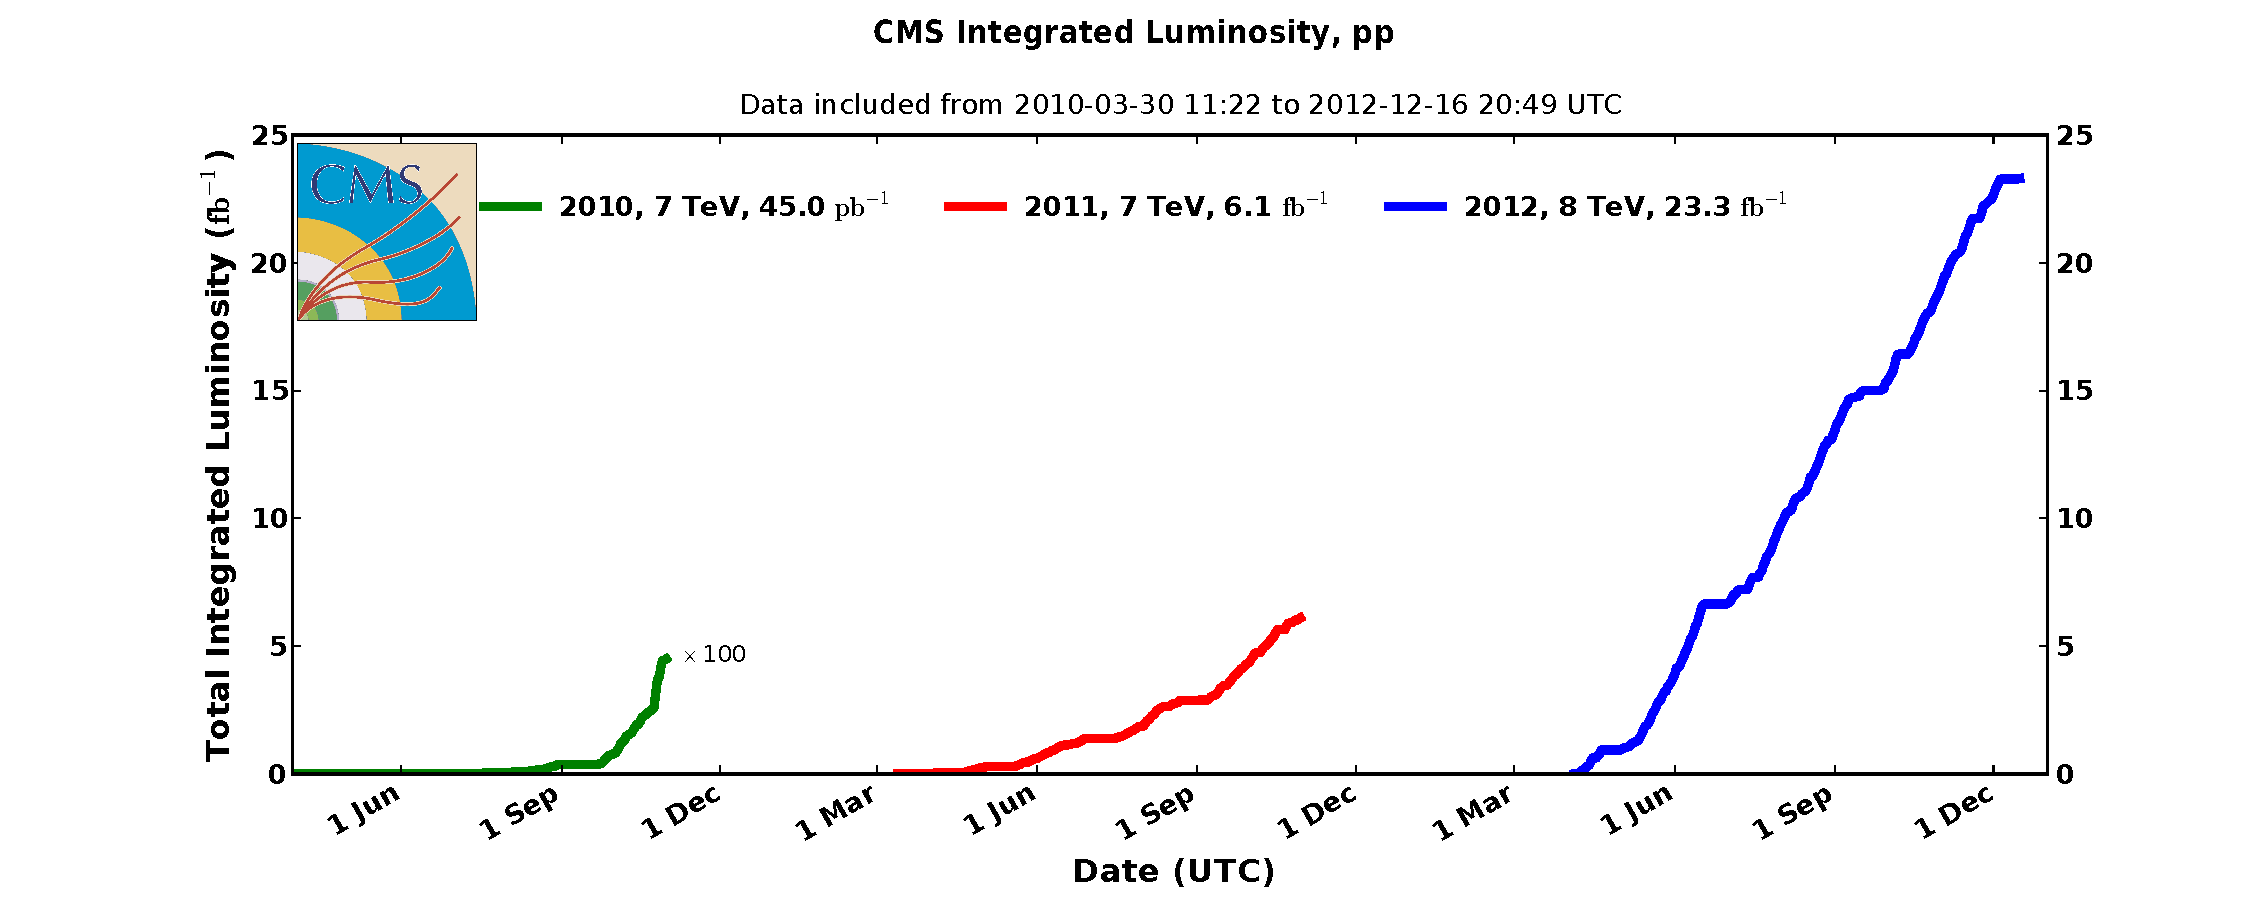
\includegraphics[width=1.00\textwidth]{Chapter02/CMS/Images/CMS_IntegratedLumi_pp_2010-2012}
  \caption{Cumulative luminosity versus day delivered to CMS during stable beams and for p-p collisions. This is shown for 2010 (green), 2011 (red) and 2012 (blue) data-taking \cite{IMAGEREF:CMSIntegratedLuminosity}.}
  \label{FIGURE:ExperimentalApparatus_CMS_IntegratedLumi_pp_2010-2012}
\end{figure}

For physics usage, data needs to undergo a certification process. In this process specialists from each \gls{CMS} subsystem check that no problem has happened during data taking that would bias or invalidate the recorded events. For 2011 a total of $5.1\,\femto\barn^{-1}$ and for 2012 a total $19.7\,\femto\barn^{-1}$ were considered of good quality for physics. 

In order to achieve high integrated luminosity \gls{LHC} collides particle bunches up to 40 million times a second, and many interactions may happen simultaneously, this effect is called \gls{PU}. Figure \ref{FIGURE:ExperimentalApparatus_CMS_PileIp_pp_2012} shows the distribution of the mean number of interaction per bunch crossing during 2012 at the \gls{CMS} experiment.

\begin{figure}[!htb]
  \centering
  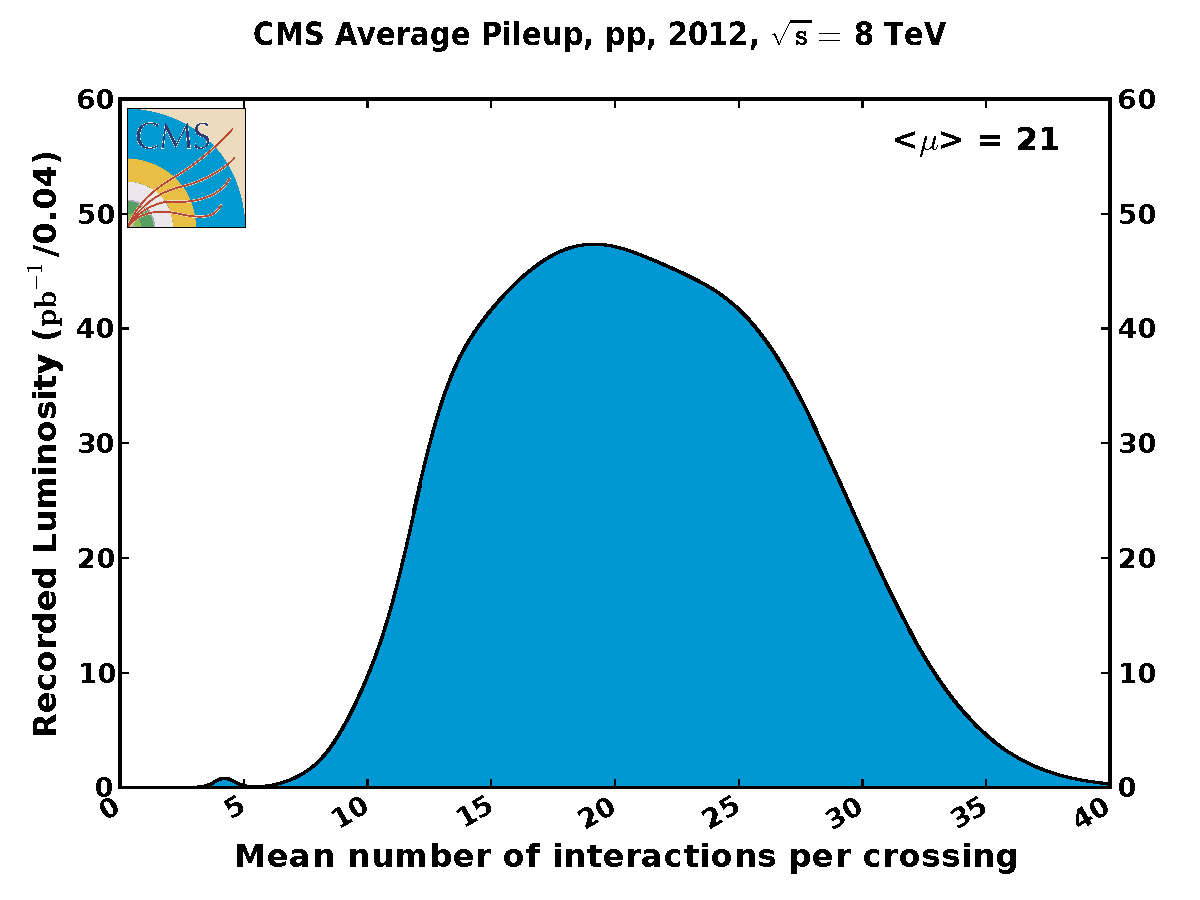
\includegraphics[width=0.60\textwidth]{Chapter02/CMS/Images/CMS_PileIp_pp_2012}
  \caption{Mean number of interactions per bunch crossing at the CMS experiment during 2012 \cite{IMAGEREF:CMSAveragePileUp2012}.}
  \label{FIGURE:ExperimentalApparatus_CMS_PileIp_pp_2012}
\end{figure}

%%%%%%%%%%%%%%%%%%%%%%%%%%%%%%%%%%%%%%%%%%%%%%%%%%%%%%%%%%%%%%%%%%%%%%%%%%%%%%%%%%%%%%%
%%% SECTION
%%%%%%%%%%%%%%%%%%%%%%%%%%%%%%%%%%%%%%%%%%%%%%%%%%%%%%%%%%%%%%%%%%%%%%%%%%%%%%%%%%%%%%%
\section{The Compact Muon Solenoid Experiment}
\label{SECTION:ExperimentalApparatus_CMS}

%Status: Done (needs review)

The \acrfull{CMS} experiment is a general purpose experiment located at the \gls{LHC} point 5, near the village of Cessy, France. It was designed to be a high performance detector studying collisions at its centre. It is composed of several subsystems in a classic onion shaped structure. A diagram of the experiment can be found in figure \ref{FIGURE:ExperimentalApparatus_CMS_Layout_Diagram}.

\begin{figure}[!htb]
  \centering
  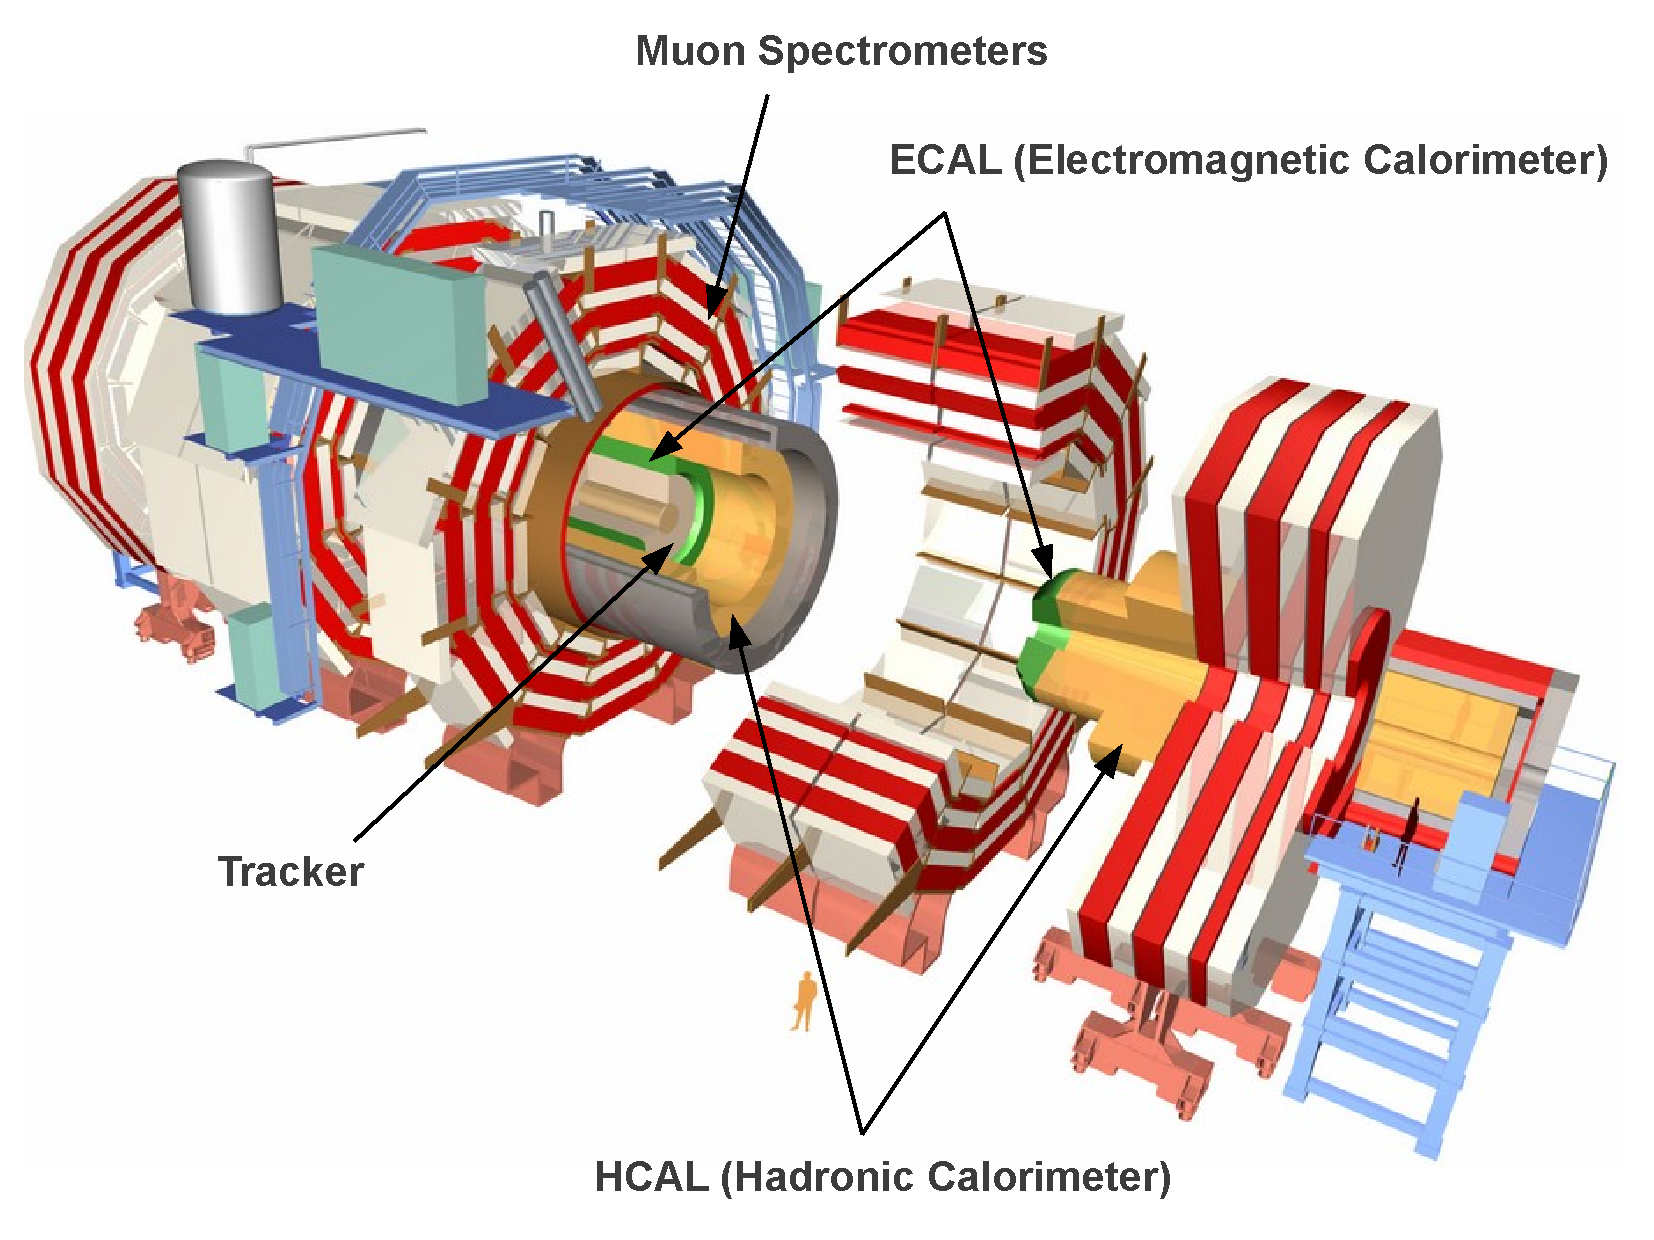
\includegraphics[width=1.00\textwidth]{Chapter02/CMS/Images/CMS_Layout_Diagram.pdf}
  \caption{Diagram of \gls{CMS} experiment showing the experiment in an open configuration and highlighting the position of its sub-detectors \cite{IMAGEREF:CERNPublic_CMSDiagram}.}
  \label{FIGURE:ExperimentalApparatus_CMS_Layout_Diagram}
\end{figure}

The main driving motivation for its design was to investigate the electroweak symmetry breaking and the Higgs mechanism at the design time was presumed to be the most likely explanation. Many alternative theories to the standard model predict new particles which could be observed at the $\TeV$ scale, \gls{CMS} as a multi-purpose experiment is well suited to search for these new scenarios. If found, such new physics may allow us to understand some of the currently open questions in particle physics, like providing a particle candidates for dark dark matter. Further more, some of these possible new physics signals could point the way towards a grand unified theory. \gls{CMS} is also capable of operating while the \gls{LHC} is colliding heavy ions and has a rich program covering the study of matter at extreme temperatures, densities and parton momentum fraction (low-x).

The requirements imposed on the \gls{CMS} design to meet its physics goals can be summarized in the following table \cite{ARTICLE:CMSTechnicalProposal,ARTICLE:TheCMSExperiment}:

\begin{itemize}
  \item Good muon identification and momentum resolution over a wide range of momenta and angles, good dimuon mass resolution ($\approx 1\%$ at $100\,GeV$), and the ability to determine un-ambiguously the charge of muons with $\pt<1\,\TeV$.
  \item Good charged-particle momentum resolution and reconstruction efficiency in the inner tracker. Efficient triggering and offline tagging of $\tau$'s and b-jets, requiring pixel detectors close to the interaction region.
  \item Good electromagnetic energy resolution, good diphoton and dielectron mass resolution ($\approx 1\%$ at $100\,\GeV$), wide geometric coverage, $\pi^0$ rejection, and efficient photon and lepton isolation at high luminosities.
  \item Good missing-transverse-energy and dijet-mass resolution, requiring hadron calorimeters with with a large hermetic geometric coverage and with fine lateral segmentation.
\end{itemize}

%TODO: Maybe re-write this!!!
The final detector design fulfils all these requirements. The experiment is compact compared to the other \gls{LHC} experiments being $22\,\meter$ long and $15\,\meter$ in diameter. Although small, it is the heaviest of the four big detectors at 12500 tonnes. Its high density is a direct consequence of it producing the highest magnetic field at $4\,\tesla$ and therefore needing more material for it to be contain in its return yoke. 

%%%%%%%%%%%%%%%%%%%%%%%%%%%%%%%%%%%%%%%%%%%%%%%%%%%%%%%%%%%%%%%%%%%%%%%%%%%%%%%%%%%%%%%
%%% SUBSECTION
%%%%%%%%%%%%%%%%%%%%%%%%%%%%%%%%%%%%%%%%%%%%%%%%%%%%%%%%%%%%%%%%%%%%%%%%%%%%%%%%%%%%
\subsection{Geometry and conventions}
\label{SECTION:ExperimentalApparatus_CMS_GeometryConventions}

% STATUS: DONE 

The adopted coordinate system has it origin in the center of \gls{CMS} where the nominal collision point is located, the \textit{y}-axis points vertically upwards, and the \textit{x}-axis points radially inward in the direction of the centre of the \gls{LHC}. The \text{z}-axis points along the beam line towards the Jura mountains from the \gls{LHC} point 5. The azimuthal angle $\phi$ is measured from the \textit{x}-axis in the \textit{x-y} plane. The polar angle $\theta$ is measured from the \textit{z}-axis.

We define pseudorapidity as $\eta = -ln(tan(\theta/2))$. All transverse quantities, like the transverse momentum ($p_\perp$), are measured in the transverse plane of beam axis. The imbalance of energy is also measured in the \textit{x-y} plane and is denoted as $E^{miss}_\perp$.

%%%%%%%%%%%%%%%%%%%%%%%%%%%%%%%%%%%%%%%%%%%%%%%%%%%%%%%%%%%%%%%%%%%%%%%%%%%%%%%%%%%%%%%
%%% SUBSECTION
%%%%%%%%%%%%%%%%%%%%%%%%%%%%%%%%%%%%%%%%%%%%%%%%%%%%%%%%%%%%%%%%%%%%%%%%%%%%%%%%%%%%
\subsection{Inner tracking system}
\label{SUBSECTION:ExperimentalApparatus_CMS_Tracker}

% STATUS: DONE (reviwed J.Pela x1)
%
% Writing points:
% * Closest detector to beam, measures trajectories of charged particles
% * With magnetic field measures momentum and charge of this particles
% * Allows vertexing (primary and secundary)
% * Different regions different occupancy
% * Final arranagement

The inner tracking system is the closest detector to the beam axis and the interaction region \cite{CMSTDR:CMSTracker,CMSTDR:CMSTrackerAddendum}. Its function is to measure the trajectory of all charged particles with momentum above 1 $\GeV$ being produced at each \gls{LHC} collision. With the help of the strong magnetic field produced by the \gls{CMS} magnet, particle trajectories are bent allowing for charge and momentum determination. With the resulting tracks is it then possible to determine the primary vertex as well as secondary vertexes like other lower energy proton-proton collision or displaced vertexes from the decay of long lived particles like B mesons.

Building a tracking system for an experiment at the \gls{LHC} is very challenging. Such system at design luminosity will be hit by an average of 1000 particles at a rate approaching $40\,\mega\hertz$. It needs to be a fast, efficient, high granularity detector, radiation hard and as thin as possible to not deflect the incoming particles trajectory. At each layer the occupancy should be of the order of $1\%$ or lower. This design requirements have lead to a tracker design entirely based on silicon detector technology. 

The volume near the interaction point can be split according to the charged particle flux into three regions:

\begin{itemize}
  \item $r<10\,\centi\meter$: highest particle flux, up to $\approx 10^8 \centi\meter^{-2}\second^{-1}$ at $r \approx 4 \centi\meter$, pixel detectors are used. The pixel size is $\approx 100 \times 150\,\micro\meter^2$, which translates into an occupancy of $10^{-4}$ per \gls{LHC} bunch crossing.
  \item $20<r<55\,\centi\meter$: particle flux decreases enough to use silicon micro-strips with a minimum cell size of $10\,\centi\meter \times 80\,\micro\meter$, leading to an occupancy of $\approx 2-3\%$ per \gls{LHC} bunch crossing.
  \item $50<r<110\,\centi\meter$: most outer region of the tracker, particle flux is low enough to use larger pitch silicon micro-strips. The maximum cell size is of $25\,\centi\meter$ $\times 180\,\micro\meter$, and occupancy is of the order of $\approx 1\%$.
\end{itemize}

The \gls{CMS} tracker final configuration is composed of a pixel detector with three barrel layers at radii between $4.4\,\centi\meter$ and $10.2\,\centi\meter$ and 2 disks on each side of the barrel. And a silicon strip tracker with 10 barrel detection layers extending up to $1.1\,\meter$ with 3 plus 9 disks on each side of the barrel. A schematic of this detector module distribution can be found at figure \ref{FIGURE:ExperimentalApparatus_CMS_Tracker_Layout}. This detector has an acceptance covering up to pseudorapidity of $|\eta|<2.5$ and has a total active area of about $200\,\meter^2$ making the largest silicon tracker ever built. 

\begin{figure}[!htb]
  \centering
  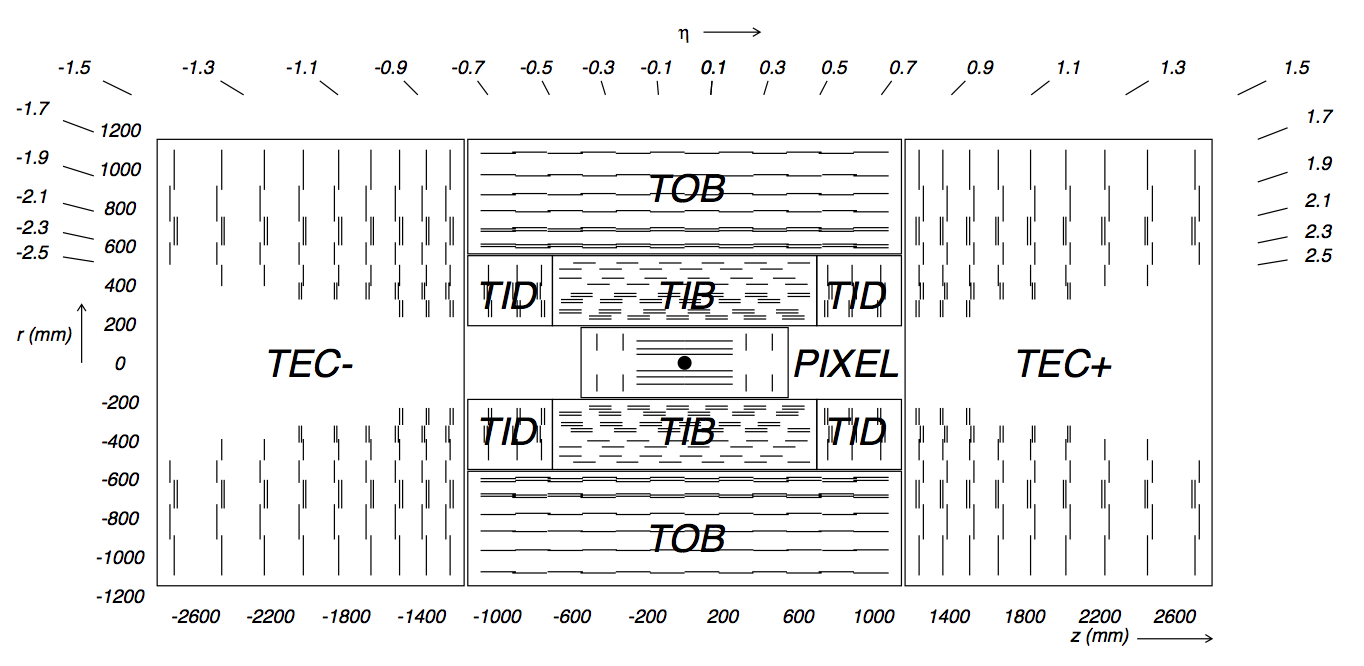
\includegraphics[width=1.0\textwidth]{Chapter02/CMS/Images/CMS_Tracker_Layout.png}
  \caption{Schematic cross section of the CMS tracker \cite{ARTICLE:TheCMSExperiment}. Each line represent a detector module. Double lines represent dual surface back-to-back detector modules. The inner tracker components are shown components: \gls{TEC}, \gls{TOB}, \gls{TID}, \gls{TIB} and Pixels. }
  \label{FIGURE:ExperimentalApparatus_CMS_Tracker_Layout}
\end{figure}

%%%%%%%%%%%%%%%%%%%%%%%%%%%%%%%%%%%%%%%%%%%%%%%%%%%%%%%%%%%%%%%%%%%%%%%%%%%%%%%%%%%%%%%
%%% SUBSECTION
%%%%%%%%%%%%%%%%%%%%%%%%%%%%%%%%%%%%%%%%%%%%%%%%%%%%%%%%%%%%%%%%%%%%%%%%%%%%%%%%%%%%
\subsection{Electromagnetic Calorimeter}
\label{SUBSECTION:ExperimentalApparatus_CMS_ECAL}

% Status: DONE (just with MSc input, and needs review)

The \gls{ECAL} is the detector responsible for measuring the energy of electrons and photons \cite{CMSTDR:CMSECAL,CMSTDR:CMSECALAddendum}. It is an hermetic energy measurement system comprised of 61200 lead tungstate ($PbWO_4$) crystals mounted in the barrel and 7324 crystals in each of the 2 endcaps and it has an acceptance up to $|\eta|<3.0$.

Lead tungstate has a fairly high density ($8.28\,\gram/\centi\meter^3$), has a short radiation length ($0.89\,\centi\meter$) and a small Moliere redius ($2.2\,\centi\meter$). The crystals also have a fast scintillation decay time emitting 80\% of the light yield in $25\,\nano\second$ (the minimal bunch crossing time at the \gls{LHC}). This characteristics make it a good choice for an electromagnetic calorimeter allowing a compact design with fine granularity. However, this crystals emit a fairly low light yield ($30\,\gamma/\MeV$) which requires the use of photo-detectors with intrinsic gain which will preform well inside a magnitic field. In the barrel region silicon \gls{APD} are used and \gls{VPT} are used in the endcaps. To guarantee good response from both crystals and \gls{APD} it is necessary to have system thermal stability, with the goal being temperature variation of less than $0.1 \celsius$.

The barrel section, the \gls{EB}, has an inner radius of $129\,\centi\meter$ and is composed of 36 identical ``supermodules'', each covers the barrel length and corresponding to a pseudo-rapidity interval of $0<|\eta|<1.479$. The crystals are quasi-projective (the axes are tilted at 3º with respect to the line from the nominal vertex position) and cover 0.0174 (i.e. 1º ) in $\Delta\phi$ and $\Delta\eta$. The crystals have a front face cross-section of $\approx 22 \times 22\,\milli\meter^2$ and a length of $230\,\milli\meter$, corresponding to 25.8 $X_0$.

The endcap section, the \gls{EE}, is at a distance of $314\,\centi\meter$ from the vertex and covering a pseudorapidity range of $1.479<|\eta|<3.0$, are each structured as 2 ``Dees'', consisting of semi-circular aluminium plates from which are cantilevered structural units of $5\times 5$ crystals, known as ``supercrystals``. A diagram of the \gls{ECAL} can be found on figure \ref{FIGURE:ExperimentalApparatus_CMS_ECAL_Layout}.

\begin{figure}[!htb]
  \centering
  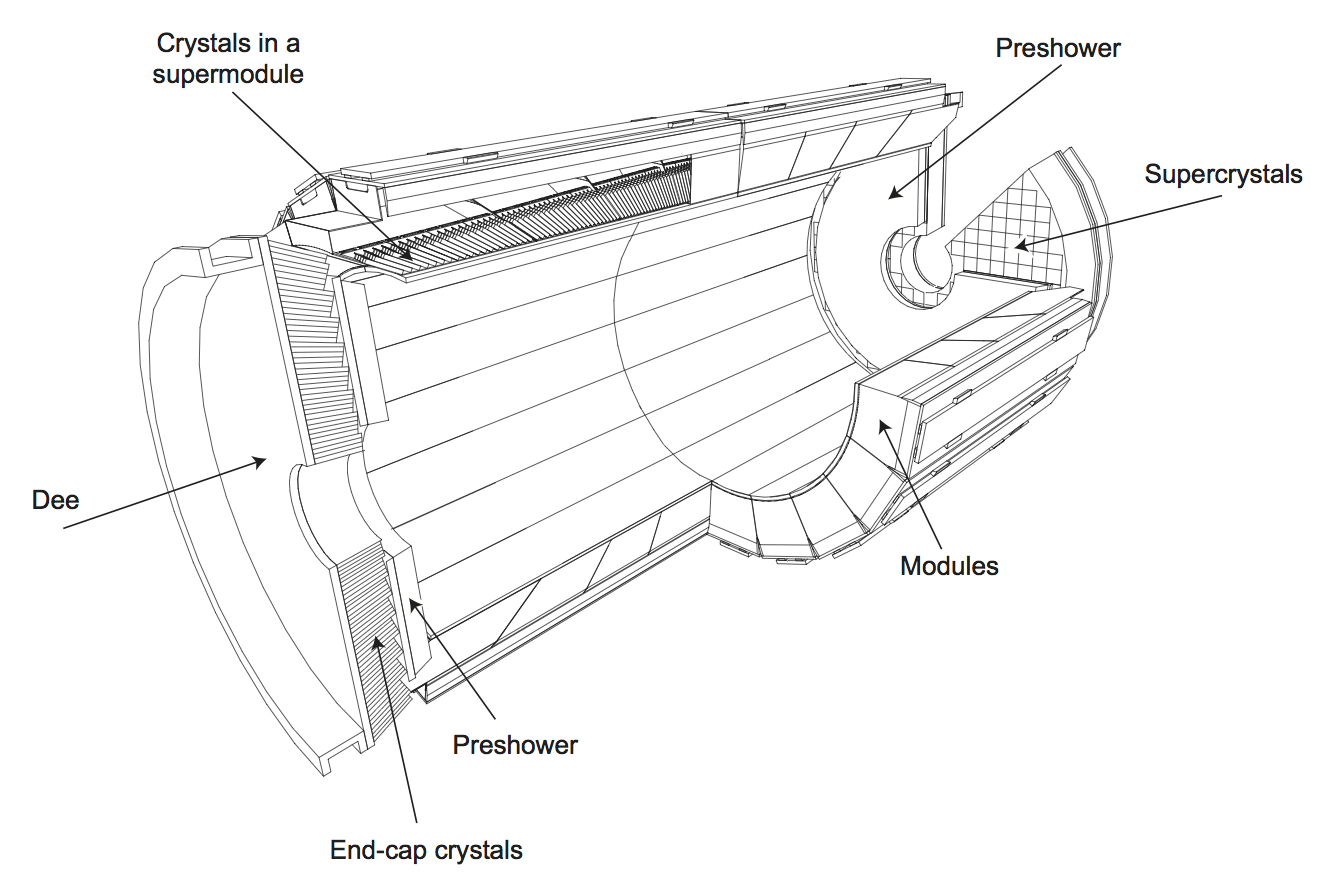
\includegraphics[width=0.8\textwidth]{Chapter02/CMS/Images/CMS_ECAL_Layout.png}
  \caption{Diagram of the ECAL layout illustrating the positions of its components \cite{ARTICLE:TheCMSExperiment}.}
  \label{FIGURE:ExperimentalApparatus_CMS_ECAL_Layout}
\end{figure}
 
The energy resolution of the \gls{ECAL} can be can be expressed as: 

\begin{equation}
\frac{\sigma}{E} = \frac{S}{\sqrt{E}} \oplus \frac{N}{E} \oplus C
\end{equation}

Here $E$ is the energy of the incoming particle, $S$ is the stochastic term which quantifies the fluctuations in scintillation and lateral containment of the shower, $N$ the noise term which relates with electronics and digitisation process and finally $C$ is a constant term that quantifies the non-uniform longitudinal response and inter-calibration errors. These parameters have been measured to be  $S=0.028\,\GeV^{1/2}$, $N=0.12\,\GeV$ and $C=0.003$ with the help of an electron beam \cite{ARTICLE:CMSECALTestBeam} and in the absence of magnetic field.

%%%%%%%%%%%%%%%%%%%%%%%%%%%%%%%%%%%%%%%%%%%%%%%%%%%%%%%%%%%%%%%%%%%%%%%%%%%%%%%%%%%%%%%
%%% SUBSUBSECTION
%%%%%%%%%%%%%%%%%%%%%%%%%%%%%%%%%%%%%%%%%%%%%%%%%%%%%%%%%%%%%%%%%%%%%%%%%%%%%%%%%%%%
\subsubsection{Preshower detector}
\label{SUBSUBSECTION:ExperimentalApparatus_CMS_ECAL_Preshower}

The \gls{CMS} Preshower is a detector locate in each endcap covering the fiducial region of $1.653<|\eta|<2.6$. Its mission is to identify neutral pions decay, help to identify electrons against minimum ionizing particles and improve electron and photon position determination.

This detector is sampling calorimeter composed by two layers of lead radiators each followed by silicon strip sensors. The lead layers have the function of forcing the incoming particles to initiate an electromagnetic shower. The first lead layer had $2X_0$ while the secong had $1X_0$, which results in 95\% of the single incident photons starting their shower before hitting the first sensor \cite{ARTICLE:TheCMSExperiment}. The shape of the lead layers edge matches the \gls{ECAL} crystal behind them to facilitate calculations at the \gls{L1T}.

Each silicon sensors have an active area of $61 \times 61\,\milli\meter$ and are $320\,\micro\meter$ thick. The sensors are divided into 32 strips each with $1.9\,\milli\meter$.  The preshower system has a total thickness of $20\,\centi\meter$ and had 137000 individual read-out channels. 

%%%%%%%%%%%%%%%%%%%%%%%%%%%%%%%%%%%%%%%%%%%%%%%%%%%%%%%%%%%%%%%%%%%%%%%%%%%%%%%%%%%%%%%
%%% SUBSECTION
%%%%%%%%%%%%%%%%%%%%%%%%%%%%%%%%%%%%%%%%%%%%%%%%%%%%%%%%%%%%%%%%%%%%%%%%%%%%%%%%%%%%
\subsection{Hadronic Calorimeter}
\label{SUBSECTION:ExperimentalApparatus_CMS_HCAL}

% STATUS: DONE

The \acrfull{HCAL} is a sampling calorimeter which is designed to measure the properties of hadron jets and indirectly neutrinos or other undiscovered particles that would result in apparent missing energy \cite{CMSTDR:CMSHCAL}. The design of the \gls{HCAL} was strongly influenced by the choice of the magnet parameters since most of the calorimetry is inside of the magnet. A diagram of the \gls{HCAL} subsystems and their location inside \gls{CMS} can be found in figure \ref{FIGURE:ExperimentalApparatus_CMS_HCAL_Layout}.

\begin{figure}[!htb]
  \centering
  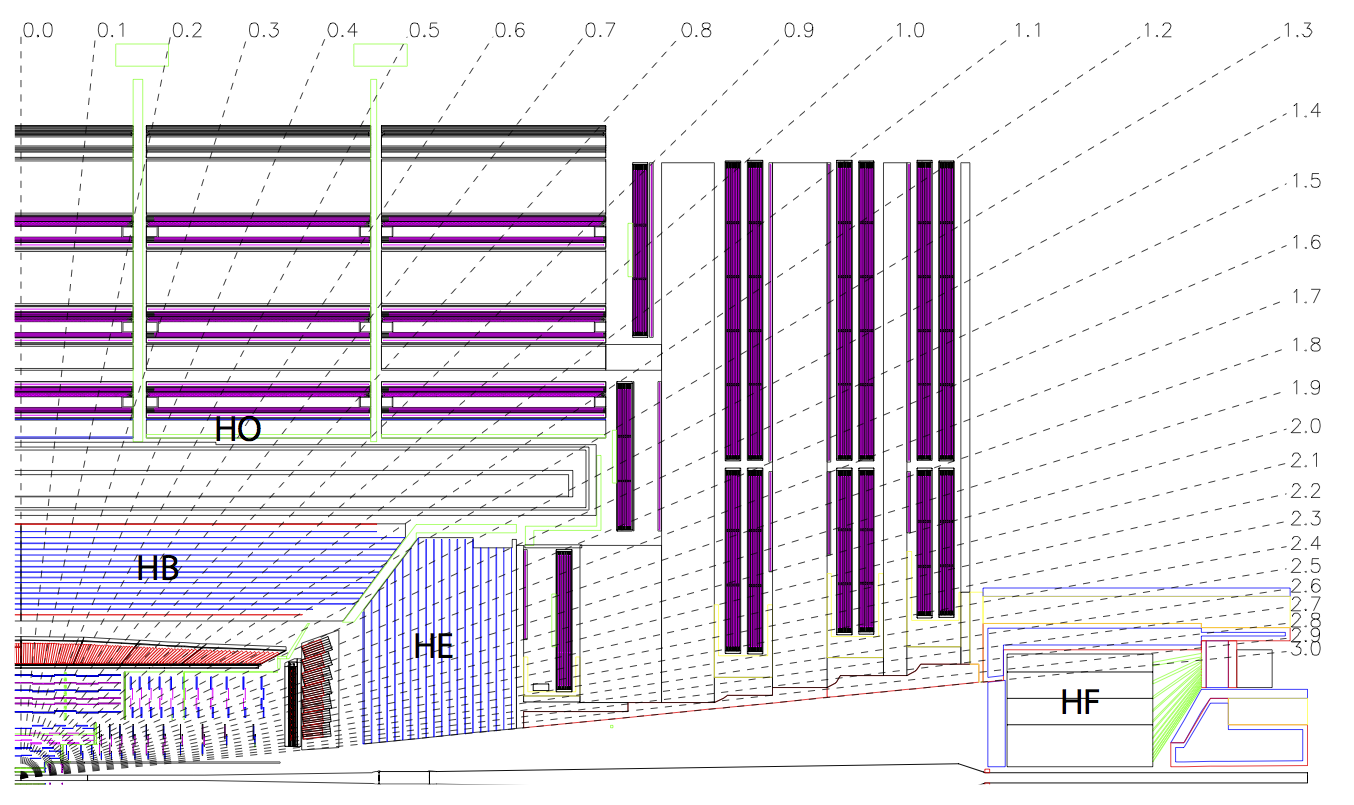
\includegraphics[width=1.0\textwidth]{Chapter02/CMS/Images/CMS_HCAL_Layout.png}
  \caption{Longitudinal view of the CMS detector highlighting the location of the \gls{HCAL} components: \gls{HB}, \gls{HE} \gls{HO} and \gls{HF} \cite{ARTICLE:TheCMSExperiment}.}
  \label{FIGURE:ExperimentalApparatus_CMS_HCAL_Layout}
\end{figure}

The \acrfull{HB} covers the region up to $|\eta|<1.3$ and is limited from the beam side by the \gls{ECAL} at radius $r=1.77\,\meter$ and outwards by the magnet at radius $r=2.95\,\meter$. This is a strict limitation on the amount of absorber material to be used. This detector is composed of 36 identical azimuthal wedges split in two half-barrels. They are constructed of brass absorber plates alternated with plastic scintillator. Brass has a short interaction length ($X_0=16.42\,\centi\meter$) and is non-magnetic. The detector is composed of 2304 towers with a segmentation of $\Delta\eta \times \Delta\phi = 0.087 \times 0.087$ which corresponds to the same area of a $5 \times 5$ arrays of \gls{ECAL} crystals.

To improve the measurement capability, an outer calorimeter, the \acrfull{HO}, is placed outside of the magnet as a \textit{tail catcher}. It increases the effective thickness of the hadronic calorimeter by over 10 interaction lengths. This detector covers the range $|\eta|<1.26$, it is composed or iron absorber and scintillator and is subdivided into sectors that cover 30º azimuthal angle in each of the barrel wheels. 

The \acrfull{HE} covers the range of $1.3<|\eta|<3.0$. It is composed by 2034 towers with a 14 towers segmentation in $\eta$ and 5º segmentation in $\phi$. The 8 inner most towers the segmentation is 10º in $\phi$, whilst the $\eta$ segmentation increases in $\eta$ from 0.09 to 0.35.

Additionally, to extend acceptance to $|\eta|<5.2$ the \gls{HF} is installed at $11.2\,\meter$ from the interaction point providing excellent hermeticity for $E_{\perp}^{miss}$ measurement. Its steel absorber is $1.65\,\meter$ deep and has quartz fibres running through it, parallel to the beam line. The energy measurement is made via Cerenkov light produced by the incoming particles inside the fibres. There are 13 tower in $\eta$ with segmentation of $\approx \Delta\eta=0.175$ except the lowest $\eta$ tower with $\approx \Delta\eta=0.1$ and highest $\eta$ tower with $\approx \Delta\eta=0.3$. The segmentation in $\phi$ is of $\Delta\phi=10º$ except in the highest $\eta$ towers which is $\Delta\phi=20º$. There are a total of tower 900 per \gls{HF} module. 

Similarly to the \gls{ECAL} the energy resolution \gls{HCAL} was tested using a test beam of single charged pions \cite{ARTICLE:CMSECALTestBeam}, and it was obtained that:

\begin{equation}
\frac{\sigma}{E} = \frac{94.3\%}{\sqrt{E}} \oplus 8.4\%.
\end{equation}

%%%%%%%%%%%%%%%%%%%%%%%%%%%%%%%%%%%%%%%%%%%%%%%%%%%%%%%%%%%%%%%%%%%%%%%%%%%%%%%%%%%%
%%% SUBSECTION
%%%%%%%%%%%%%%%%%%%%%%%%%%%%%%%%%%%%%%%%%%%%%%%%%%%%%%%%%%%%%%%%%%%%%%%%%%%%%%%%%%%%
\subsection{Solenoid Magnet}
\label{SUBSECTION:ExperimentalApparatus_CMS_Magnet}

%Status: DONE

The design requirements for correct charge assignment and \pt determination for charge particles and specially muons drive the magnet parameters choice. For muons, unambiguously charge determination requires momentum resolution of $\Delta p/p \approx 10\%$ at $p = 1 \TeV$. This requirements are specially difficult to obtain in the forward regions but with the correct length/radius ratio can be obtained with a modestly sized solenoid magnet but with large field \cite{CMSTDR:CMSPhysicsVol1,CMSTDR:CMSMagnet}.

The choice of the \gls{CMS} collaboration was to build a Niobium-Titanium (NbTi) superconducting solenoid magnet which has been design to operate at fields up to $4\,\tesla$ it has a diameter of $6\,\meter$ and a length of $12.5\,\meter$ at maximum field the stored energy reaches $2.7\,\giga\joule$. Typically, the magnet is only run at $3.8\,\tesla$ in order to maximize its lifetime. To contain such an enormous magnetic flux a $10\,\kilo\ton$ return yoke envelopes the magnet with 5 wheels in the barrel region and 2 endcaps composed of 3 disks closing the sides \cite{ARTICLE:TheCMSExperiment}. A summary of the most important magnet parameters can be found at table \ref{TABLE:ExperimentalApparatus_CMSMagnetParameters}.

\begin{table}[!htb]
  \centering
  \begin{tabular}{|l|c|}
  \hline
  Parameter & Value \\
  \hline\hline
  Field           & 4 T \\
  Inner Bore      & 5.9 m \\
  Length          & 12.9 m \\
  Number of turns & 2168 \\
  Current         & 19.5 kA \\
  Stored Energy   & 2.7 GJ \\
  Hoop Stress     & 64 atm \\
  \hline
  \end{tabular}
  \caption[Parameters of the CMS superconducting solenoid]{Parameters of the CMS superconducting solenoid}
  \label{TABLE:ExperimentalApparatus_CMSMagnetParameters}
\end{table}


%%%%%%%%%%%%%%%%%%%%%%%%%%%%%%%%%%%%%%%%%%%%%%%%%%%%%%%%%%%%%%%%%%%%%%%%%%%%%%%%%%%%
%%% SUBSECTION
%%%%%%%%%%%%%%%%%%%%%%%%%%%%%%%%%%%%%%%%%%%%%%%%%%%%%%%%%%%%%%%%%%%%%%%%%%%%%%%%%%%%
\subsection{Muon System}
\label{SUBSECTION:ExperimentalApparatus_CMS_Moun}

%Status: DONE (needs review)

The muon detection is an important part of the mission of \gls{CMS} \cite{CMSTDR:CMSMuonSystem}. Muons are fairly easy to detect when compared with other elementary particles and are only rarely produced in proton-proton collisions. To take the example of the \gls{SM} Higgs boson, while the decay mode involving a pair of Z bosons is fairly unlikely compared with other decays the Z bosons can decay into 4 mouns. This decay while rare does not have significant backgrounds making it a ''golden channel`` for discovery, which indeed was proven the case \cite{ARTICLE:CMSHiggsObservation}. Many other models, like SUSY, use muon final states in their searches exactly for the same reason. The \gls{CMS} muon system is composed of 3 types of gaseous detectors depending on they location and momentum reconstruction needs. A diagram of the disposition of this system inside \gls{CMS} can be found on figure \ref{FIGURE:ExperimentalApparatus_CMS_Muon_Layout}.

\begin{figure}[!htb]
  \centering
  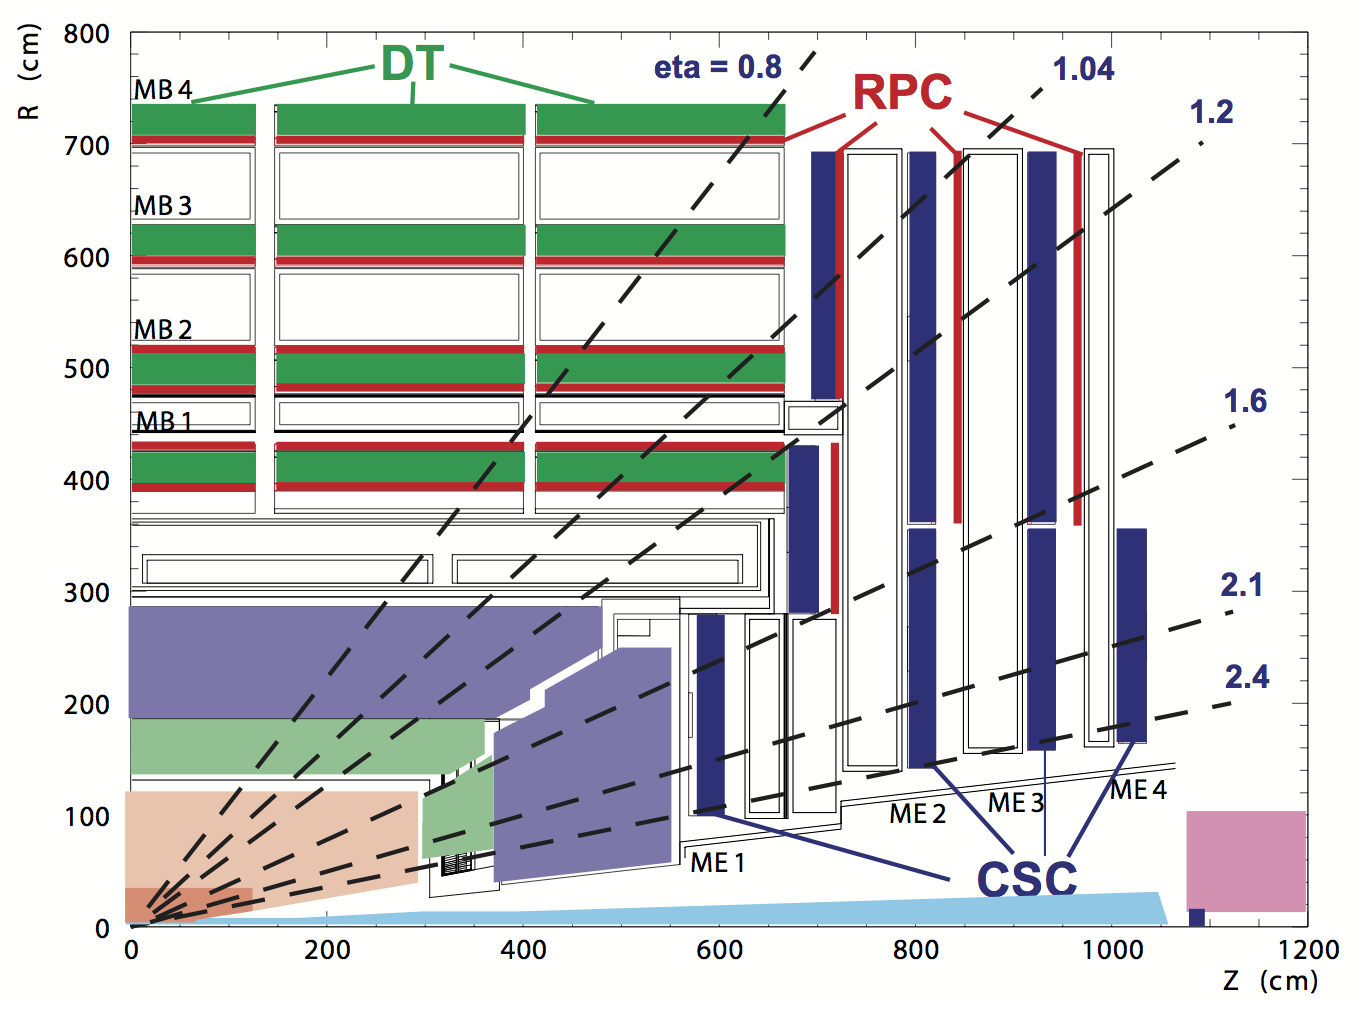
\includegraphics{Chapter02/CMS/Images/CMS_Muon_Layout.png}
  \caption{Diagram of the \gls{CMS} muon systems. The location of each muon chamber for each subsystem is showed \cite{CMSTDR:CMSPhysicsVol1}.}
  \label{FIGURE:ExperimentalApparatus_CMS_Muon_Layout}
\end{figure}

In the barrel and up to $|\eta|<1.2$, \gls{DT} are used. since the neutron background is small and the field is constant. This system is composed 250 chambers and is arranged in 4 concentric cylindrical layers which are installed inside of the return yoke. This chambers have a total of 172000 wires with a length of $2.4\,\meter$ which are housed inside of tubes filled with a mixture of argon and carbon-dioxide. Each of the wheels of the barrel is split into 12 sectors covering 30º azimuthal angle. The maximum gas ionization drift is of $2.0\,\centi\meter$ and results in a single point resolution is $\approx 200\,\micro\meter$ per wire. For each station each measured muon the $\phi$ resolution is better than $200\,\micro\meter$ and direction resolution is $\approx 1\,\milli\radian$.

In the endcaps \gls{CSC} are used in the region between $2.4>|\eta|>0.9$. Here, muon and background rates are high and the magnetic field is not uniform. This system has fast response and is radiation resistant. It is composed by 468 chambers arranged in 4 stations per side. Each chamber is trapezoidal in shape and made of 6 gas gaps and covers either 10º or 20º in $\phi$. Each gap contains a plane of cathode strips and a plane of anode wires. For each chamber the spacial resolution is of the order of $200\,\micro\meter$ and the angular resolution is $\approx 10\,\milli\radian$ in $\phi$.

Finally the \gls{RPC} covers the $|\eta|<1.6$ range. This system overlaps with the 2 other muon systems. It is very fast with an ionization event being much faster than the bunch crossing time. This fast response allows, in conjunction with a dedicated trigger system, to select the correct bunch crossing associated with the detection of a muon. In the barrel there 480 rectangular chambers arranged in 4 stations with 6 \gls{RPC} layers (2 layers are present in the 2 stations closest to the beam pipe). In the endcaps there are 3 \gls{RPC} disk shaped stations on each side, which are composed by trapezoidal shaped detectors.

The combined muon system offline momentum resolution is of the order of 9\% for small values of $\eta$ and $p$ and for transverse momenta of up to $200\,\GeV$. At higher energies of around $1\,\TeV$ the standalone momentum resolution is in the range of 15-40\% depending on $|\eta|$. This values are limited by the muon multiple-scattering before arriving to the muon system. If we combine the tracker information into a global fit the resolution for lower \pt tracks improves an order of magnitude while at higher momenta (around $1\,\TeV$) it is of about 5\%, which is well inside the \gls{CMS} design requirements.

%%%%%%%%%%%%%%%%%%%%%%%%%%%%%%%%%%%%%%%%%%%%%%%%%%%%%%%%%%%%%%%%%%%%%%%%%%%%%%%%%%%%%%%
%%% SUBSECTION
%%%%%%%%%%%%%%%%%%%%%%%%%%%%%%%%%%%%%%%%%%%%%%%%%%%%%%%%%%%%%%%%%%%%%%%%%%%%%%%%%%%%
\subsection{Data Acquisition System}
\label{SUBSECTION:ExperimentalApparatus_CMS_DAQ}

%Status: DONE (needs review)

The \gls{CMS} \gls{DAQ} system is designed to process, analyse and ultimately store the information collected by the detector \cite{CMSTDR:CMSTridasTDRVol2}. The \gls{LHC} produces bunch crossings at a rate of $40\,\mega\hertz$ but we are only capable of storing between $10^2-10^3$ events per second. At design luminosity each collision will have an average of over 20 simultaneous collisions and produce a zero-suppressed data payload of around $1\,\mega\byte$. To reduce the event rate to completely retrieve from the detector buffers a first level of trigger was developed. This hardware system reduces the amount of events to be processed to a maximum of $100 \kilo\hertz$. Even with this event suppression the \gls{DAQ} has to retrieve and move $\approx 100\, \giga\byte\second^{-1}$ from the detector to the surface. This data comes from approximately 650 data sources and has to be merged into a single event package. The information is then passed to a computer farm where a software filters serve as a second level of trigger. In this system the event rate is further reduced up top a factor of 1000 making the output rate compatible with what can be saved into permanent storage. A diagram of this system can be found on figure \ref{FIGURE:ExperimentalApparatus_CMS_DAQ_Diagram}.

\begin{figure}[!htb]
  \centering
  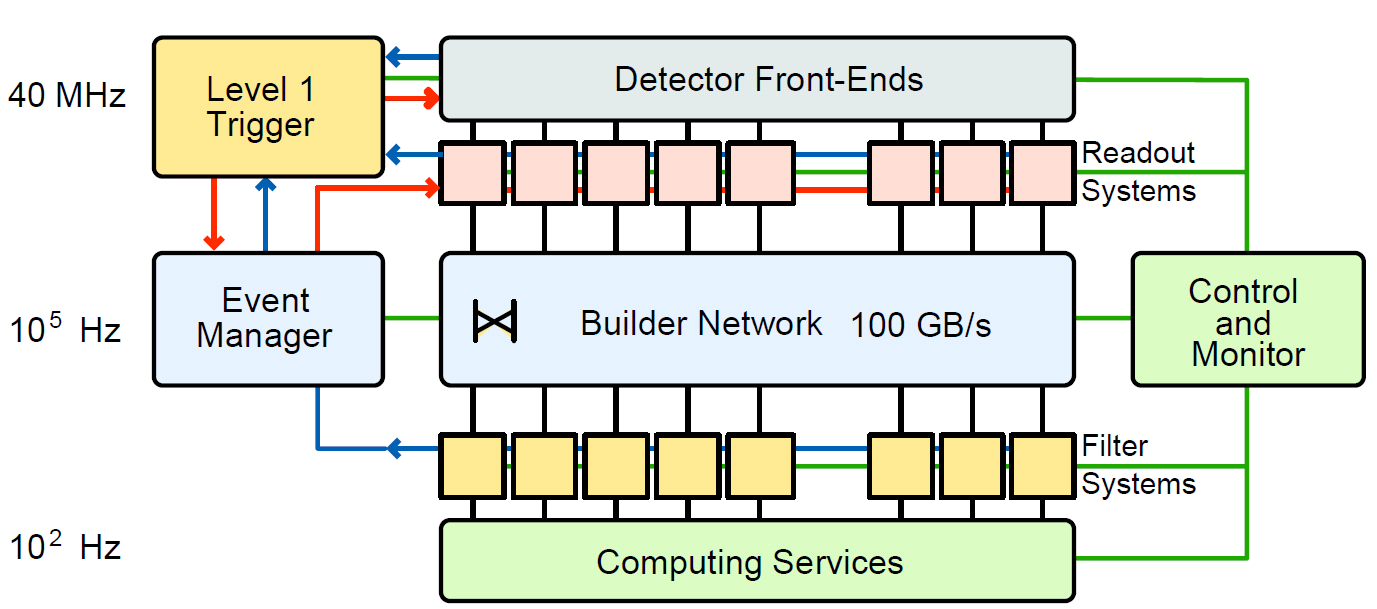
\includegraphics[width=0.80\textwidth]{Chapter02/CMS/Images/CMS_DAQ_Diagram.png}
  \caption{Diagram of the \gls{CMS} \gls{DAQ} system. Data flow is showed as the lines connecting each electronics or computing units \cite{ARTICLE:TheCMSExperiment}.}
  \label{FIGURE:ExperimentalApparatus_CMS_DAQ_Diagram}
\end{figure}

%%%%%%%%%%%%%%%%%%%%%%%%%%%%%%%%%%%%%%%%%%%%%%%%%%%%%%%%%%%%%%%%%%%%%%%%%%%%%%%%%%%%%%%
%%% SUBSECTION
%%%%%%%%%%%%%%%%%%%%%%%%%%%%%%%%%%%%%%%%%%%%%%%%%%%%%%%%%%%%%%%%%%%%%%%%%%%%%%%%%%%%
\subsection{Trigger System}
\label{SUBSECTION:ExperimentalApparatus_CMS_Trigger}

%Status: DONE (needs review)

As described on the previous section the \gls{CMS} trigger system is responsible for selecting which collisions are recorded in real-time. We can only save $10^2-10^3$ events per second with the current systems. This implies that the trigger system needs to obtain a data reduction of a factor of $\mathcal{O}(10^6-10^7)$. This is achieved with a two level trigger system, the first is a dedicated hardware system named \acrfull{L1T} \cite{CMSTDR:CMSTridasTDRVol1} and the second is a commercial computer system running dedicated software called the \acrfull{HLT} \cite{CMSTDR:CMSTridasTDRVol2}.

Initially, all data is stored for 128 bunch crossing which corresponds to $3.2\,\micro\second$. This is the time we have to make a first decision to keep or discard an event. This is the task of the \gls{L1T} which has the target to reduced the data to a maximum rate of $100\,\kilo\hertz$. There isn't enough time to get all the information from the detector, so only a coarse version of the calorimetry and muon systems data, and some correlation between them is accessed. With this information the \gls{L1T} produces a set of particle candidates and energy sums over which custom user defined algorithms can use to filter events. A diagram of the \gls{L1T} trigger components and the data flow across the system is present on figure \ref{FIGURE:ExperimentalApparatus_CMS_L1T_Layout}.

\begin{figure}[!htb]
  \centering
  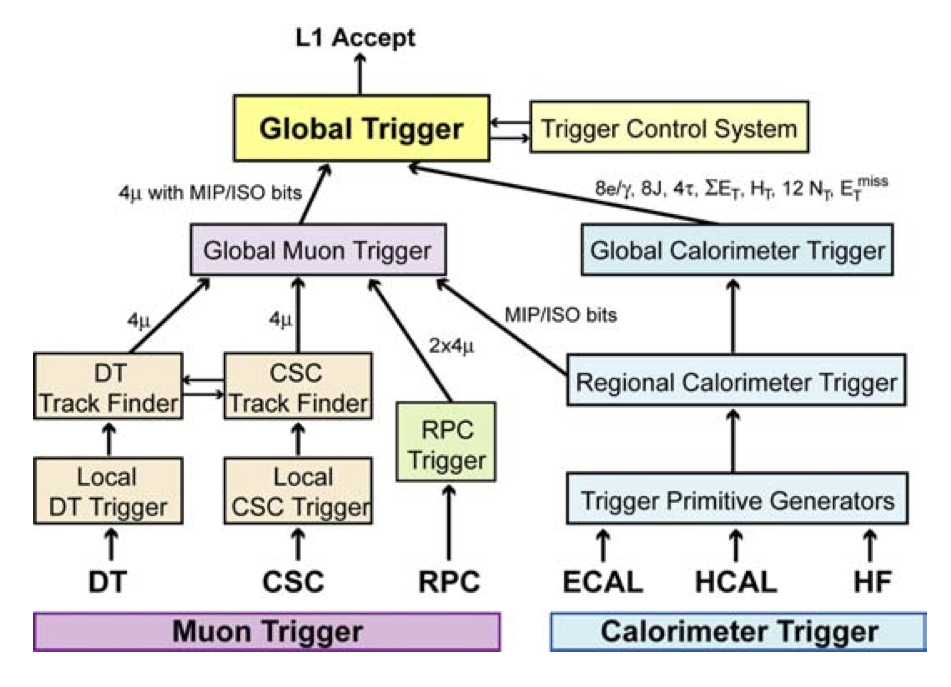
\includegraphics[width=0.80\textwidth]{Chapter02/CMS/Images/CMS_L1T_Layout.png}
  \caption{Diagram of the \gls{L1T} system. The arrows indicate data flow and the number of particle candidates at each step is indicate \cite{ARTICLE:TheCMSExperiment}.}
  \label{FIGURE:ExperimentalApparatus_CMS_L1T_Layout}
\end{figure}

The \gls{HLT} receives events accepted by the \gls{L1T} and needs to perform further event reduction of 
$\mathcal{O}(10^{3}-10^{2})$ to a final output rate of $\mathcal{O}(10^{2-3})\,\hertz$ . This system is composed of standard computing hardware in the form of computing farm with $\approx 15\,\kilo$ \gls{CPU}. This system, using the additional latency created by the \gls{L1T} event selection, is able to make use of the complete detector information including the tracker data. More sophisticated and precise algorithms are therefore possible which can be tailored to select any desired physical final state. 

Event selection algorithms at both the \gls{L1T} and \gls{HLT} are frequently updated during data taking. The selection thresholds may be tuned in order to control the rate with the changes of \gls{LHC} luminosity. Novel methods or strategies to identify particles more efficiently can be implemented, like \gls{PU} subtraction or new calibrations. Analysis groups may also show interest in recording new event final final states for which new selection criteria may be developed. The set of algorithms used for data taking is normally referred as the \textit{trigger menu}. 

After events pass both levels of the trigger they are recorded into permanent storage. During 2012-13 operation, two output streams were saved. The \textit{prompt data stream}, with a rate of approximately $300\,\hertz$, was composed of high priority trigger paths which were immediately reconstructed. And the \textit{parked data stream}, with an average rate of $600\,\hertz$, was stored without reconstruction. This data waited until computing resources were  free to go through reconstruction \cite{ARTICLE:CMSDataParking}. This process was finalised a few months after the \gls{LHC} Run I was finished.

Even with such measures to reduce the data to be stored, each \gls{LHC} experiment records several petabytes of data every year in addition to similarly sized amounts of simulated events.

%%%%%%%%%%%%%%%%%%%%%%%%%%%%%%%%%%%%%%%%%%%%%%%%%%%%%%%%%%%%%%%%%%%%%%%%%%%%%%%%%%%%%%%
%%% SUBSECTION
%%%%%%%%%%%%%%%%%%%%%%%%%%%%%%%%%%%%%%%%%%%%%%%%%%%%%%%%%%%%%%%%%%%%%%%%%%%%%%%%%%%%
\subsection{Computing}
\label{SUBSECTION:ExperimentalApparatus_CMS_Computing}

%Status: DONE

The quantity of data produced by the \gls{LHC} and the necessary processing capability is so big that it would be difficult to have all computing resources in a single place. For this reason a tiered system was developed, where all participating computing sites are connected and have specific roles and responsibilities in the data taking, processing and storing. This global computing system is know as the Grid \cite{CMSTDR:CMSComputing}.

The \gls{CERN} Data Centre is the Tier 0 of this network, all data produced by the \gls{LHC} experiments is handled by this facility. Only about 20\% of the total capacity of the Grid is hosted here, but \gls{CERN} Tier 0 has the very important mission of safe keeping all the raw data produced by the experiments. It also has the task of doing the first attempt of event reconstruction, which is the process identifying meaningful physics objects in data.

There are 7 \gls{CMS} Tier 1 computer centres around the world. They are responsible to store a proportional amount of raw and reconstructed data. If any reprocessing of the data is needed, this centres are responsible for this task and storing the resulting output as well. Tier 1 centres also host simulated data and distribute it to Tier 2 centres. 

Local research centres like universities of scientific laboratories are normally at the Tier 2 level. This centres have the responsibility of handling a proportional share of simulated data production and reconstruction. Currently there are over 150 Tier 2 centres around the world

Individual computers or local clusters without any formal engagement with the Grid structure, are considered to be the Tier 3 level of the Grid. 

%%%%%%%%%%%%%%%%%%%%%%%%%%%%%%%%%%%%%%%%%%%%%%%%%%%%%%%%%%%%%%%%%%%%%%%%%%%%%%%%%%%%%%%
%%% SUBSECTION
%%%%%%%%%%%%%%%%%%%%%%%%%%%%%%%%%%%%%%%%%%%%%%%%%%%%%%%%%%%%%%%%%%%%%%%%%%%%%%%%%%%%
\subsection{Level 1 Trigger: Stage I Upgrade}
\label{SUBSECTION:ExperimentalApparatus_CMS_L1TStage1}

%Status: Writing

An extensive upgrade program for the \gls{L1T} electronics was planed and is being executed in order to cope with the increase of luminosity and pile-up predicted for the period after \gls{LS1} \cite{CMSTDR:CMSL1Upgrade,CMSTDR:CMSUpgradeTDR}. The center-of-mass energy has almost double from $8\,\TeV$ to $13\,\TeV$, instantaneous luminosity will also increase as will average pile-up. Also, the bunch separation has change from $50\,\nano\second$ to $25\,\nano\second$ making out-of-time pile-up a significant problem. 

To ensure physics performance during 2015 and beyond only a partial upgrade was executed for the 2015 run which is known as the \textit{Stage-1} upgrade. The main feature of this upgrade program is the replacement of the existing \gls{GCT}. Two key enhancements were possible: 

\begin{itemize}
  \item Event-by-event pile-up energy subtraction for jets reconstruction, $e/\gamma$ isolation, $\tau$ isolation.
  \item Smaller feature size $\tau$ candidates, which will have significantly better energy estimation and background rejection.
\end{itemize}

The intermediate system will have significantly better performance than the now legacy system. The full 2016 calorimeter trigger system will additionally provide finer granularity which will lead to increased position and energy resolution. 

  \chapter{Physics Objects and Monte Carlo simulation}

\section{Physics objects definition}

\subsection{Electron}

\subsection{Muon}

\subsection{Tau}

\subsection{Jets}

\subsection{Missing Transverse Energy}

\section{Monte Carlo simulation}



% \clearpage
% \section{Introduction}

The search for an invisible decay of a vector boson produced Higgs boson was first made public with CMS Physics Analysis Summary (PAS) HIG-13-013 which was further improved and combined with other Higgs boson production channel in the CMS paper HIG-13-30. Additional support material can be found at the CMS Analysis Notes (AN) AN-2012/403\cite{CMS_AN_2013-403} and AN-2013/205.

During the 2012 data taking run two main streams of data were recorded. The main stream with an event rate of the order of 300 Hz to be promptly reconstructed and made available for analysis in a few days after being recorded, this dataset is referred to as the prompt data. The secondary stream with lower trigger thresholds with an event rate of the order of 1kHz which would only be reconstructed when the computing resources would be available outside of the data taking period, dataset is referred to as parked data. Our previous results
were produced using the prompt data only and this work now extends on previous work by using the now available parked data. Since this dataset has been recorded with lower trigger thresholds the analysis was re-optimised to take advantage of this new available phase space. The details of the newly developed analysis can be found in CMS AN-14-243\cite{CMS_AN_2014-243}.

It is normally a requirement for many CMS publications to have a cross check analysis implemented independently from the main result in order to be able to ensure accuracy of the final results due to possible errors with the software implementation. For this purpose the previous prompt data VBF Higgs to Invisible results and publication were produced by two different and independent code frameworks and before publication a good level of synchronization were obtained. Due to lack of man power and time it was decide for the 2012 parked data analysis to only proceed with a single framework. At a later stage of the analysis it was thought that at least some level of cross check would be a good measure to limit the possibility of implementation errors and to allow extra confidence on the final results.

This cross check analysis starts from the same ntuples produced by the main analysis which were produced over all the relevant datasets and are recorded with data formats also used by other analysis at Imperial College London, e.g. both the SM and MSSM Higgs to $\tau\bar{\tau}$, the Higgs to $\tau\bar{\tau}b\bar{b}$ and prompt Higgs to invisible analyses. No cuts are applied at ntuple production except the official CMS selection for good usable data using the appropriate golden JSON file.

From those initial ntuple an independent code framework was developed in order to replicate all relevant numbers and plots from the main analysis.

% \section{Data samples}

For this analysis we used the proton-proton collision parked data collected by the CMS experiment during 2012-13. An analysis purposely constructed trigger was used to collect this data.

\begin{table}[htp]
\centering

\begin{tabular}{|l|c|}
\hline
Dataset & $\int{Luminosity}$ $[pb^{-1}]$ \\
\hline \hline
/MET/Run2012A-22Jan2013-v1/AOD        & 889 \\
/VBF1Parked/Run2012B-22Jan2013-v1/AOD & 3871 \\
/VBF1Parked/Run2012C-22Jan2013-v1/AOD & 7152 \\
/VBF1Parked/Run2012D-22Jan2013-v1/AOD & 7317 \\
\hline
Total analysed & 19229 \\
\hline \hline
Total certified luminosity & 19789 \\
\hline
\end{tabular}

\caption{Used datasets and their respective integrated luminosities after applying certified for physics filtering. Each dataset corresponds to a recording period/era of the 2012-13 data acquisition run.}
\end{table}

% Review text abouve

% To include
% * Explain breifly the validadion process (JSON)
% * Table with data included


% \section{Event Filters and object definitions}

%STATUS: Finished
%TODO: 
% * Could not find any reference to this recommendations!
\subsection{Vertex}

The interaction point is normally assumed to be the reconstructed  primary vertex, defined as the vertex with highest sum of associated tracks \pt squared, or if that cannot be determined the beam spot position is assumed. Knowing precisely the interaction point will allow to determine object quantities relative to it which allow for better object identification and pile-up control. At least one good vertex implicitly required by tracking failure event quality filter. And Additionally we require explicitly that a good vertex is reconstructed with the following characteristics. 

\begin{itemize}
  \item NOT(isFake): We require a real reconstructed vertex from tracks, not the beam spot.
  \item Number of degrees of freedom: $n_{dof}>4$
  \item Longitudinal distance: $|z|<=24$
  \item Radial distance to beam line: $d_{xy}<2$
\end{itemize}

%STATUS: Finished
%TODO: 
% * Add citation for the Jet-MET POG for this filter usage (include data and page version)
% * QUESTION: Should I include description of what each filter does?
\subsection{Event quality filters}

During data recording issues may happen with the detector or acquisition which may render some of the events unusable. The groups responsible for each part of the detector and physics object check the data after and was taken and if they find such problems software event filters are made available for analysis to be able to remove this problematic events. This event filters will address issues like detector know problems, miss firing of calibration sequences or failure to reconstruct physics objects. The Jet-MET Particle Object Group (POG) recommends the usage of the following filters which are used in this analysis\cite{CMS:JetMETPOG:MissingETOptionalFilters}.

\begin{itemize}
  \item CSCTightHaloFilter
  \item HBHENoiseFilter
  \item EcalDeadCellTriggerPrimitiveFilter
  \item trackingFailureFilter
  \item eeBadScFilter
  \item ECAL Laser filter (via event list)
  \item HCAL Laser filter (via event list)
\end{itemize}

In turn the JetMET group recommend the usage of the following Tracking POG Filter\cite{CMS:TrackingPOG:TrackingPOGFilters}:

\begin{itemize}
  \item  logErrorTooManyClusters
  \item  manystripclus53X
  \item  toomanystripclus53X
\end{itemize}

The event rejection efficiencies from the all filters except ECAL and HCAL laser event filters can be found at table \ref{table_EventQualityFilterEff}. This values are measured the vertex requirements. 

\begin{table}[!htp]
\centering

\begin{tabular}{|l||c|c|c|c|}
\hline
Filter                  & Prompt A & Parked B & Parked C & Parked D \\
\hline \hline
ECAL Laser Filter       & 0.928521 & 0.008659 & 0.000000 & 0.000000 \\
HCAL Laser Filter       & 0.007258 & 0.000000 & 0.000270 & 0.000000 \\
\hline
ECAL+ HCAL Laser Filter & 0.935704 & 0.008659 & 0.000270 & 0.000000 \\
\hline
\end{tabular}

\caption{Event rejection efficiency for the ECAL and HCAL Laser Filters. This events have to be removed due to the untimely firing of the calibration laser for this systems.}
\label{table_CaloLaserFilterEff}
\end{table}


The values for the ECAL and HCAL laser event filters are present in table \ref{table_CaloLaserFilterEff}. This value are calculated after vertex requirement and the filters in table \ref{table_EventQualityFilterEff}. 

\begin{table}[htp]
\centering

\begin{tabular}{|l||c|c|c|c|}
\hline
Filter                             & Prompt A  & Parked B & Parked C & Parked D \\
\hline \hline
HBHENoiseFilter                    & 22.900905 & 0.190670 & 0.187739 & 0.170753 \\
EcalDeadCellTriggerPrimitiveFilter &  0.375381 & 0.009300 & 0.010206 & 0.012526 \\
eeBadScFilter                      &  0.007852 & 0.000001 & 0.000000 & 0.000009 \\
trackingFailureFilter              &  3.073876 & 0.000328 & 0.007464 & 0.000290 \\
manystripclus53X                   &  0.001829 & 0.001319 & 0.002335 & 0.001327 \\
toomanystripclus53X                &  0.000484 & 0.001149 & 0.002006 & 0.001173 \\
logErrorTooManyClusters            &  0.000027 & 0.000009 & 0.000021 & 0.000016 \\
CSCTightHaloFilter                 & 10.263068 & 0.398497 & 0.402936 & 0.508025 \\
\hline
Total                              & 28.501208 & 0.598417 & 0.601999 & 0.689380 \\
\hline
\end{tabular}

\caption{Percentage of events in data failing each of the event quality filters after requesting on good vertex. For the parked analysis we use prompt A and parked B, C and D datasets.}
\label{table_EventQualityFilterEff}
\end{table}

It is observed that the HBHENoiseFilter vetos around 22\% of the event for prompt run A but this behaviour is not observed in any of the parked datasets. This specific filter removed events with noise in the HCAL. An example of noise would be a ``hot tower'' reading very high energy values, some times for several events. Since this energy will not be balance in each event this will greatly increase \MET. On the prompt dataset there are \MET only triggers which were fired in such events which then get removed by this filter, those triggers are not present in parked dataset. This can clearly be seen if we apply first our trigger selection (Jets+\MET) and then recalculate the event rejection efficiencies, this values can be found in table \ref{table_EventQualityFilterEff_PostTrigger}.

\begin{table}[htp]
\centering

\begin{tabular}{|l||c|c|c|c|}
\hline
Filter                             & Prompt A & Parked B & Parked C & Parked D \\
\hline \hline
HBHENoiseFilter                    & 1.264571 & 0.186895 & 0.178422 & 0.154080 \\
EcalDeadCellTriggerPrimitiveFilter & 0.572468 & 0.010081 & 0.010338 & 0.010725 \\
eeBadScFilter                      & 0.000989 & 0.000001 & 0.000000 & 0.000000 \\
trackingFailureFilter              & 0.062289 & 0.000401 & 0.009729 & 0.000231 \\
manystripclus53X                   & 0.002966 & 0.001264 & 0.002304 & 0.001255 \\
toomanystripclus53X                & 0.002966 & 0.001093 & 0.001955 & 0.001103 \\
logErrorTooManyClusters            & 0.000000 & 0.000000 & 0.000000 & 0.000000 \\
CSCTightHaloFilter                 & 0.400431 & 0.397531 & 0.403156 & 0.506917 \\
\hline                             
Total                              & 2.201877 & 0.594332 & 0.592977 & 0.671026 \\
\hline
\end{tabular}

\caption{Percentage of events in data failing each of the event quality filters after requesting on good vertex and trigger conditions. For the parked analysis we use prompt A and parked B, C and D datasets.}
\label{table_EventQualityFilterEff_PostTrigger}
\end{table}

Both tables \ref{table_EventQualityFilterEff} and \ref{table_CaloLaserFilterEff} can be directly compared with the values produced by the main analysis and presented in AN-14-243\cite{CMS_AN_2014-243}. No differences are observed.

%STATUS: In progress
%TODO:  
\subsection{Jets}

In this analysis we use particle flow  jets clustered with the $anti-k_{T}$ algorithm with a cone size of 0.5. 

The correction L1FastJet, L2Relative and L3Absolute are applied to both data and monte carlo (MC) and additionally we apply L2L3Residual to data.

The to correct Jet Energy Scale we apply global tag FT53\_V21A\_AN6::All for data and START53\_V27::All for monte carlo.

The jets with this characteristics and corrections are available in the ntuples produced by the main analysis as the "standard" jets collection. We further require that our selected jets pass PFJet ID and pileup ID. And we clean the jet collection by removing all jets that closer then $\Delta R < 0.5$ to any veto electron or loose muon (relevant for control regions).

%Out of this jets we select the ones passing loose PFJet ID and pileup ID. We also clean the jet collection by removing all jets that closer then %$\Delta R < 0.5$% to any veto electron or loose muon (relevant for control regions).
 
%% FOR MY PHD THESIS 
%% Details on 
%  
% As a selection condition for out jets we use the PFJet ID described at [[CMS/JetID.Recommendations_for_8_TeV_data_a][JetID page]].
% 
% The jet requirements are:
%    * Neutral Hadron Fraction %$ <0.99 $%
%    * Neutral EM Fraction %$ <0.99 $%
%    * Number of Constituents  %$ >1 $%
% Additionally for %$|\eta| < 2.4$% we require:
%    * Charged Hadron Fraction %$  >0 $%
%    * Charged Multiplicity %$ >0 $%
%    * Charged EM Fraction %$ 0.99 $%
% 
% ---+++ Pileup ID 
% 
% Using the prescription at the [[CMS.PileupJetID][PileupJetID page]] we reject pileup jets cutting at loose working point of a BDT with Dec2012 weights and package recojets/jetproducers with version METPU_5_3_X_v4. The computation of the MVA value per jet is made when the ntuples are produced and this values are stored within each jet. We cut on the BDT score categorizing in %$p_{\perp}$% and %$|\eta|$% as follows:
% 
% %BEGINLATEX%
% \begin{tabular}{|c|c|c|}
% \hline
% Jet $p_{\perp}$ & Jet $|\eta|$ & $BDT_{score}$ \\
% \hline \hline
% $20 < p_{\perp} \leq 30$ & $|\eta| < 2.5$ & $BDT_{score} > -0.80$ \\
% $20 < p_{\perp} \leq 30$ & $2.50 \leq |\eta| < 2.75$ & $BDT_{score} > -0.85$ \\
% $20 < p_{\perp} \leq 30$ & $2.75 \leq |\eta| < 3.00$ & $BDT_{score} > -0.84$ \\
% $20 < p_{\perp} \leq 30$ & $3.00 \leq |\eta| < 5.00$ & $BDT_{score} > -0.85$ \\
% $30 < p_{\perp}$ & $|\eta| < 2.5$ & $BDT_{score} > -0.80$ \\
% $30 < p_{\perp}$ & $2.50 \leq |\eta| < 2.75$ & $BDT_{score} > -0.74$ \\
% $30 < p_{\perp}$ & $2.75 \leq |\eta| < 3.00$ & $BDT_{score} > -0.68$ \\
% $30 < p_{\perp}$ & $3.00 \leq |\eta| < 5.00$ & $BDT_{score} > -0.77$ \\
% \hline
% \end{tabular}
% %ENDLATEX%

%STATUS: In progress
%TODO:  
\subsection{Missing transverse energy \texorpdfstring{(\MET)}{}}


%STATUS: In progress
%TODO: 
% Convert base cut based ID to a table  
\subsection{Electrons}

% Make citation for CMS.EgammaCutBasedIdentification
For this analysis we use two categories of electrons "veto electrons" and "tight electrons". Both this categories of particles are based on standard EGamma POG cut based object definition which can be found at (TODO:CITATION). Additionally, we require some additional cuts to each category (TODO:WHY).

\subsubsection{Veto electrons}
 
The "veto electrons" are defined by the base requirements of the cut based electron ID veto working point of the EGamma POG with some additional cuts on top. 
 
Requirements of the cut based electron ID veto working point:

Barrel Cuts ( $ |\eta_{supercluster}|<=1.479 $ )
\begin{itemize}
  \item $ | \Delta\eta(track,supercluster) | < 0.007 $
  \item $ | \Delta\phi(track,supercluster) | < 0.8 $
  \item $ \sigma(i\eta,i\eta) < 0.01 $
  \item $ H/E < 0.15 $
  \item $ |d_{0}(vertex)| < 0.04 $
  \item $ |d_{Z}(vertex)| < 0.2 $
  \item $ \frac{PF_{isolation}}{p_{\perp}} < 0.15 $ for $ \Delta R_{cone}=0.3 $
\end{itemize}

Endcap Cuts ( $ 1.479 < |\eta_{supercluster}| < 2.5 $ )
\begin{itemize}
  \item $ | \Delta\eta(track,supercluster) | < 0.1 $
  \item $ | \Delta\phi(track,supercluster) | < 0.7 $
  \item $ \sigma(i\eta,i\eta) < 0.03 $
  \item $ |d_{0}(vertex)| < 0.04 $
  \item $ |d_{Z}(vertex)| < 0.2 $
  \item $ \frac{PF_{isolation}}{p_{\perp}} < 0.15 $ for $ \Delta R_{cone}=0.3 $
\end{itemize}

Additional requirements for this analysis
\begin{itemize}
  \item $ p_{\perp} > 10 $ GeV
  \item $ |\eta| < 2.4 $
  \item $ Effective-Area-Corrected-Isolation < 0.15 $ (is stated in the note as additional requirement but does not look like it is)
  \item $d_{xy}<0.04$ cm (is stated in the note as additional requirement but does not look like it is)
  \item $d_{z} < 0.2 $ cm (is stated in the note as additional requirement but does not look like it is)
\end{itemize}

\subsubsection{Tight electrons}

The "tight electrons" are defined by using the base requirements of the cut based electron ID tight working point (similar to 2011 very tight WP70) of the EGamma POG with some additional cuts on top.
 
Requirements of the cut based electron ID tight working point (similar to 2011 very tight WP70):

Barrel Cuts ( $ |\eta_{supercluster}|<=1.479 $ )
\begin{itemize}
  \item $ | \Delta\eta(track,supercluster) | < 0.004 $
  \item $ | \Delta\phi(track,supercluster) | < 0.3  $
  \item $ \sigma(i\eta,i\eta) < 0.01 $
  \item $ H/E < 0.12 $
  \item $ |d_{0}(vertex)| < 0.02 $
  \item $ |d_{Z}(vertex)| < 0.1 $
  \item $ |\frac{1}{E}-\frac{1}{p}| < 0.05 $
  \item $ \frac{PF_{isolation}}{p_{\perp}} < 0.10 $ for $ \Delta R_{cone}=0.3 $
  \item Conversion rejection: vertex fit probability: 1e-6
  \item Conversion rejection: missing hits $<= 0$
\end{itemize}

Endcap Cuts ( $ 1.479 < |\eta_{supercluster}| < 2.5 $ )
\begin{itemize}
  \item $ | \Delta\eta(track,supercluster) | < 0.005 $
  \item $ | \Delta\phi(track,supercluster) | < 0.2  $
  \item $ \sigma(i\eta,i\eta) < 0.03 $
  \item $ H/E < 0.10 $
  \item $ |d_{0}(vertex)| < 0.02 $
  \item $ |d_{Z}(vertex)| < 0.1 $
  \item $ |\frac{1}{E}-\frac{1}{p}| < 0.05 $
  \item $ \frac{PF_{isolation}}{p_{\perp}} < 0.10(0.07) $ for $ p_{\perp} > 20 (p_{\perp} <= 20) $ and $ \Delta R_{cone}=0.3 $
  \item Conversion rejection: vertex fit probability: 1e-6
  \item Conversion rejection: missing hits $<= 0$
\end{itemize}

Additional requirements for this analysis:
\begin{itemize}
  \item $ p_{\perp} > 20 $ GeV
  \item $ |\eta| < 2.4 $
  \item $ Effective-Area-Corrected-Isolation < 0.10 $
  \item $d_{xy}<0.02 $ cm
  \item $d_{z} < 0.1 $ cm
\end{itemize}


%STATUS: In progress
%TODO: 
\subsection{Muons}




%STATUS: In progress
%TODO: 
\subsection{Taus}


% \section{Signal selection}

\subsection{Pre-selection}

\begin{table}[!htp]
\centering

\begin{tabular}{|l||c|c|c|c|}
\hline
Filter                  & Prompt A & Parked B & Parked C & Parked D \\
\hline \hline
ECAL Laser Filter       & 0.928521 & 0.008659 & 0.000000 & 0.000000 \\
HCAL Laser Filter       & 0.007258 & 0.000000 & 0.000270 & 0.000000 \\
\hline
ECAL+ HCAL Laser Filter & 0.935704 & 0.008659 & 0.000270 & 0.000000 \\
\hline
\end{tabular}

\caption{Event rejection efficiency for the ECAL and HCAL Laser Filters. This events have to be removed due to the untimely firing of the calibration laser for this systems.}
\label{table_CaloLaserFilterEff}
\end{table}


\begin{table}[htp]
\centering

\begin{tabular}{|l|c|c|c|c||c|}
\hline
 & \rotatebox{90}{Prompt Run A} & \rotatebox{90}{Parked Run B} & \rotatebox{90}{Parked Run C} & \rotatebox{90}{Parked Run D} & \rotatebox{90}{Total Data} \\
\hline \hline
Vertex Filter & 3606391 & 132346320 & 228049748 & 308041846 & 672044305 \\
Event Quality Filters & 2658960 & 131554431 & 226680352 & 305918529 & 666812272 \\
ECAL Laser Filter & 2634271 & 131543040 & 226680352 & 305918529 & 666776192 \\
HCAL Laser Filter & 2634080 & 131543040 & 226679741 & 305918529 & 666775390 \\
L1T ETM Filter & 2461217 & 88174347 & 160560859 & 227801622 & 478998045 \\
HLT Filter & 97522 & 75100422 & 137527238 & 152041761 & 364766943 \\
$N(Electrons_{veto})=0$ & 96600 & 74947192 & 137241812 & 151725585 & 364011189 \\
$N(Muon_{loose})=0$ & 94864 & 74913002 & 137179173 & 151652654 & 363839693 \\
Dijet cut & 28164 & 23666926 & 43292391 & 42218637 & 109206118 \\
MET cut & 6252 & 57929 & 102384 & 120600 & 287165 \\
$MET_{Significance}$ cut & 3828 & 24179 & 42683 & 41620 & 112310 \\
$Min(\Delta\phi(MET,jets))$ cut & 405 & 1824 & 3452 & 3374 & 9055 \\
\hline
\end{tabular}
\caption{Event Yield for the Pre-Selection Region.}
\end{table}


\begin{table}[!htp]
\centering

\begin{tabular}{|l|c|c|c|}
\hline
Dataset & Main Analysis & Cross Check Analysis & $\frac{CC}{Main}-1$ \\ 
\hline \hline
Prompt A &  405 &  405 & 0.00\% \\
Parked B & 1824 & 1824 & 0.00\% \\
Parked C & 3453 & 3452 & -0.03 \% \\
Parked D & 3374 & 3374 & 0.0\% \\
\hline \hline
Total & 9056 & 9055 & -0.01\% \\
\hline
\end{tabular}

\caption{Comparison between main and cross check analysis for the event yield of the event pre-selection. There is a difference of a single event between both analysis which is a difference in total yield around 0.01\%.}
\end{table}


\subsection{Signal region}

\begin{table}[htp]
\centering

\begin{tabular}{|l|c|c|c|c||c|}
\hline
 & \rotatebox{90}{Prompt Run A} & \rotatebox{90}{Parked Run B} & \rotatebox{90}{Parked Run C} & \rotatebox{90}{Parked Run D} & \rotatebox{90}{Total Data} \\
\hline \hline
Vertex Filter & 3606391 & 132346320 & 228049748 & 308041846 & 672044305 \\
Event Quality Filters & 2658960 & 131554431 & 226680352 & 305918529 & 666812272 \\
ECAL Laser Filter & 2634271 & 131543040 & 226680352 & 305918529 & 666776192 \\
HCAL Laser Filter & 2634080 & 131543040 & 226679741 & 305918529 & 666775390 \\
L1T ETM Filter & 2461217 & 88174347 & 160560859 & 227801622 & 478998045 \\
HLT Filter & 97522 & 75100422 & 137527238 & 152041761 & 364766943 \\
$N(Electrons_{veto})=0$ & 96600 & 74947192 & 137241812 & 151725585 & 364011189 \\
$N(Muon_{loose})=0$ & 94864 & 74913002 & 137179173 & 151652654 & 363839693 \\
Dijet cut & 18338 & 13678405 & 25090291 & 24082304 & 62869338 \\
MET cut & 4167 & 38178 & 68047 & 79723 & 190115 \\
$MET_{Significance}$ cut & 786 & 3396 & 5988 & 5567 & 15737 \\
$Min(\Delta\phi(MET,jets))$ cut & 34 & 91 & 205 & 178 & 508 \\
\hline
\end{tabular}
\caption{Event Yield for the Signal Region.}
\end{table}


\begin{table}[!htp]
\centering

\begin{tabular}{|l|c|c|c|}
\hline
Dataset & Main Analysis & Cross Check Analysis & $\frac{CC}{Main}-1$ \\ 
\hline \hline
Prompt A &  34 &  34 & 0.00\% \\
Parked B &  91 &  91 & 0.00\% \\
Parked C & 205 & 205 & 0.00 \% \\
Parked D & 178 & 178 & 0.00\% \\
\hline \hline
Total & 508 & 508 & 0.00\% \\
\hline
\end{tabular}

\caption{Comparison between main and cross check analysis for the event yield of signal region. No difference in yields is observed either in total or by acquisition era.}
\end{table}

% \section{Background estimation}

\subsection{W to \texorpdfstring{electron+\MET}{electron+MET}}

The selection consists of the following cuts:

\begin{itemize}
  \item Vertex cut
  \item Event quality filters (MET Filters)
  \item ECAL+HCAL Laser filters
  \item L1T ETM Filter (L1T\_ETM40 emulation)
  \begin{itemize}
    \item $ L1T\_ETM >= 40 $
  \end{itemize}
  \item HLT path filter
  \begin{itemize}
    \item From run 190456 to 193621 (Run 2012 A) use HLT\_DiPFJet40\_PFMETnoMu65\_MJJ800VBF\_AllJets* 
    \item From run 193833 to 196531 (Run 2012 B) use HLT\_DiJet35\_MJJ700\_AllJets\_DEta3p5\_VBF*
    \item From run 198022 to 203742 (Run 2012 C) use HLT\_DiJet35\_MJJ700\_AllJets\_DEta3p5\_VBF*
    \item From run 203777 to 208686 (Run 2012 D) use HLT\_DiJet30\_MJJ700\_AllJets\_DEta3p5\_VBF*
  \end{itemize}
  \item Exactly one $Electron_{Veto}$
  \begin{itemize}
    \item Using veto electron defined on this page
  \end{itemize}
  \item Exactly one $Electron_{Tight}$
  \begin{itemize}
    \item Using tight electron defined on this page
  \end{itemize}
  \item Muon Veto
  \begin{itemize}
    \item Using veto muons defined on this page (to be done)
  \end{itemize}
  \item $ MET > 90 $ GeV
  \item $ MET_{significance} > 4.0 $
  \item Dijet cut (leading dijet requirements):
  \begin{itemize}
    \item Lead dijet $ p_{\perp} > 50$ GeV
    \item Sub-lead dijet $ p_{\perp} > 45$ GeV
    \item Jets $ |\eta| < 4.7 $
    \item Dijet $ \Delta\eta < 3.6 $
    \item Dijet $ m_{jj} > 1200 $ GeV
  \end{itemize}
  \item $ Min(\Delta\phi(MET,Jet_{p_{\perp}>30})))>2.3 $
\end{itemize}

\begin{table}[!htp]
\centering

\begin{tabular}{|l|c|c|c|c||c|}
\hline
 & \rotatebox{90}{Prompt Run A} & \rotatebox{90}{Parked Run B} & \rotatebox{90}{Parked Run C} & \rotatebox{90}{Parked Run D} & \rotatebox{90}{Total Data} \\
\hline \hline
Vertex Filter & 3606391 & 132346320 & 228049748 & 308041846 & 672044305 \\
Event Quality Filters & 2658960 & 131554431 & 226680352 & 305918529 & 666812272 \\
ECAL Laser Filter & 2634271 & 131543040 & 226680352 & 305918529 & 666776192 \\
HCAL Laser Filter & 2634080 & 131543040 & 226679741 & 305918529 & 666775390 \\
L1T ETM Filter & 2461217 & 88174347 & 160560859 & 227801622 & 478998045 \\
HLT Filter & 97522 & 75100422 & 137527238 & 152041761 & 364766943 \\
$N(Electrons_{veto})=1$ & 899 & 151621 & 282481 & 312807 & 747808 \\
$N(Muon_{loose})=0$ & 852 & 151249 & 281801 & 312033 & 745935 \\
$N(Electrons_{tight})=1$ & 398 & 23751 & 44323 & 50279 & 118751 \\
Dijet cut & 64 & 1607 & 3145 & 3077 & 7893 \\
MET cut & 55 & 281 & 543 & 525 & 1404 \\
$MET_{Significance}$ cut & 31 & 123 & 242 & 197 & 593 \\
$Min(\Delta\phi(MET,jets))$ cut & 4 & 16 & 24 & 24 & 68 \\
\hline
\end{tabular}

\caption{Electron+MET Yields}
\end{table}


\begin{table}[!htp]
  \centering
  
\begin{tabular}{|l|c|c||c|}
  \hline
  Dataset & Main Analysis & Cross Check Analysis & $\frac{CC}{Main}-1$ \\ 
  \hline \hline
  Prompt Run A &  4 &  4 & 0.00\% \\
  Parked Run B & 16 & 16 & 0.00\% \\
  Parked Run C & 24 & 24 & 0.00\% \\
  Parked Run D & 24 & 24 & 0.00\% \\
  \hline \hline
  Total & 68 & 68 & 0.00\% \\
  \hline
\end{tabular}

\caption{Comparison between main and cross check analysis for the event yield of Electron+MET event selection. No difference in yields is observed either in total or by acquisition era.}
\end{table}

\subsection{W to \texorpdfstring{$\mu$+\MET}{muon+MET}}

The selection consists of the following cuts
\begin{itemize}
  \item Vertex cut 
  \item Event quality filters (MET Filters)
  \item ECAL+HCAL Laser filters
  \item L1T ETM Filter (L1T\_ETM40 emulation)
  \begin{itemize}
    \item $ L1T\_ETM >= 40 $
  \end{itemize}
  \item HLT path filter
  \begin{itemize}
    \item From run 190456 to 193621 (Run 2012 A) use HLT\_DiPFJet40\_PFMETnoMu65\_MJJ800VBF\_AllJets* 
    \item From run 193833 to 196531 (Run 2012 B) use HLT\_DiJet35\_MJJ700\_AllJets\_DEta3p5\_VBF*
    \item From run 198022 to 203742 (Run 2012 C) use HLT\_DiJet35\_MJJ700\_AllJets\_DEta3p5\_VBF*
    \item From run 203777 to 208686 (Run 2012 D) use HLT\_DiJet30\_MJJ700\_AllJets\_DEta3p5\_VBF*
  \end{itemize}
  \item Electron Veto
  \begin{itemize}
    \item Using veto electron defined on this page
  \end{itemize}
  \item Exactly one $Muon_{loose}$
  \begin{itemize}
    \item Using veto muons defined on this page (to be done)
  \end{itemize}
  \item Exactly one $Muon_{tight}$
  \begin{itemize}
    \item Using veto muons defined on this page (to be done)
  \end{itemize}
  \item $MET > 90 $ GeV
  \item $MET_{significance} > 4.0 $
  \item Dijet cut (leading dijet requirements):
  \begin{itemize}
    \item Lead dijet $ p_{\perp} > 50$ GeV
    \item Sub-lead dijet $ p_{\perp} > 45$ GeV
    \item Jets $ |\eta| < 4.7 $
    \item Dijet $ \Delta\eta < 3.6 $
    \item Dijet $ m_{jj} > 1200 $ GeV
  \end{itemize}
  \item $ Min(\Delta\phi(MET,Jet_{p_{\perp}>30})))>2.3 $
\end{itemize}

\begin{table}[!htp]
\centering

\begin{tabular}{|l|c|c|c|c||c|}
\hline
 & \rotatebox{90}{Prompt Run A} & \rotatebox{90}{Parked Run B} & \rotatebox{90}{Parked Run C} & \rotatebox{90}{Parked Run D} & \rotatebox{90}{Total Data} \\
\hline \hline
Vertex Filter & 3606391 & 132346320 & 228049748 & 308041846 & 672044305 \\
Event Quality Filters & 2658960 & 131554431 & 226680352 & 305918529 & 666812272 \\
ECAL Laser Filter & 2634271 & 131543040 & 226680352 & 305918529 & 666776192 \\
HCAL Laser Filter & 2634080 & 131543040 & 226679741 & 305918529 & 666775390 \\
L1T ETM Filter & 2461217 & 88174347 & 160560859 & 227801622 & 478998045 \\
HLT Filter & 97522 & 75100422 & 137527238 & 152041761 & 364766943 \\
$N(Electrons_{veto})=0$ & 96600 & 74947192 & 137241812 & 151725585 & 364011189 \\
$N(Muon_{loose})=1$ & 1625 & 33505 & 61325 & 71449 & 167904 \\
$N(Muon_{tight})=1$ & 1223 & 9662 & 17873 & 20088 & 48846 \\
Dijet cut & 176 & 1493 & 2740 & 2684 & 7093 \\
MET cut & 157 & 809 & 1545 & 1493 & 4004 \\
$MET_{Significance}$ cut & 86 & 487 & 910 & 825 & 2308 \\
$Min(\Delta\phi(MET,jets))$ cut & 10 & 60 & 124 & 106 & 300 \\
\hline
\end{tabular}
\caption{Muon+MET Region}
\end{table}


\begin{table}[!htp]
\centering

\begin{tabular}{|l|c|c||c|}
  \hline
  Dataset & Main Analysis & Cross Check Analysis & $\frac{CC}{Main}-1$ \\ 
  \hline \hline
  Prompt Run A &  10 &  10 & 0.00\% \\
  Parked Run B &  60 &  60 & 0.00\% \\
  Parked Run C & 124 & 124 & 0.00\% \\
  Parked Run D & 106 & 106 & 0.00\% \\
  \hline \hline
  Total & 300 & 300 & 0.00\% \\
  \hline
\end{tabular}

\caption{Comparison between main and cross check analysis for the event yield of Muon+MET event selection. No difference in yields is observed either in total or by acquisition era.}
\end{table}

\subsection{W to \texorpdfstring{$\tau$+\MET}{tau+MET}}

\begin{table}[!htp]
\centering

\begin{tabular}{|l|c|c|c|c||c|}
\hline
 & \rotatebox{90}{Prompt Run A} & \rotatebox{90}{Parked Run B} & \rotatebox{90}{Parked Run C} & \rotatebox{90}{Parked Run D} & \rotatebox{90}{Total Data} \\
\hline \hline
Vertex Filter & 3606391 & 132346320 & 228049748 & 308041846 & 672044305 \\
Event Quality Filters & 2658960 & 131554431 & 226680352 & 305918529 & 666812272 \\
ECAL Laser Filter & 2634271 & 131543040 & 226680352 & 305918529 & 666776192 \\
HCAL Laser Filter & 2634080 & 131543040 & 226679741 & 305918529 & 666775390 \\
L1T ETM Filter & 2461217 & 88174347 & 160560859 & 227801622 & 478998045 \\
HLT Filter & 97522 & 75100422 & 137527238 & 152041761 & 364766943 \\
$N(Electrons_{veto})=0$ & 96600 & 74947192 & 137241812 & 151725585 & 364011189 \\
$N(Muon_{loose})=0$ & 94864 & 74913002 & 137179173 & 151652654 & 363839693 \\
Dijet cut & 18338 & 13678405 & 25090291 & 24082304 & 62869338 \\
MET cut & 4167 & 38178 & 68047 & 79723 & 190115 \\
$MET_{Significance}$ cut & 786 & 3396 & 5988 & 5567 & 15737 \\
$N(Tau)=1$ & 12 & 47 & 63 & 59 & 181 \\
$M_{perp}(MET,\tau)$ cut & 5 & 35 & 46 & 38 & 124 \\
$Min(\Delta\phi(MET,Dijet))$ cut & 2 & 22 & 25 & 27 & 76 \\
\hline
\end{tabular}
\caption{Event Yield for the Tau+MET Region.}
\end{table}


\begin{table}[!htp]
\centering

\begin{tabular}{|l|c|c||c|}
  \hline
  Dataset & Main Analysis & Cross Check Analysis & $\frac{CC}{Main}-1$ \\ 
  \hline \hline
  Prompt Run A &  2 &  2 & 0.00\% \\
  Parked Run B & 22 & 22 & 0.00\% \\
  Parked Run C & 25 & 25 & 0.00\% \\
  Parked Run D & 27 & 27 & 0.00\% \\
  \hline \hline
  Total & 76 & 76 & 0.00\% \\
  \hline
\end{tabular}

\caption{Comparison between main and cross check analysis for the event yield of Tau+MET event selection. No difference in yields is observed either in total or by acquisition era.}
\end{table}

\subsection{Z to \texorpdfstring{$\mu\mu$}{mumu}}

The selection consists of the following cuts:
\begin{itemize}
  \item Vertex cut
  \item Event quality filters (MET Filters)
  \item ECAL+HCAL Laser filters
  \item !L1T ETM Filter (L1T\_ETM40 emulation)
  \begin{itemize}
    \item $ L1T\_ETM >= 40 $
  \end{itemize}
  \item HLT path filter
  \begin{itemize}
    \item From run 190456 to 193621 (Run 2012 A) use HLT\_DiPFJet40\_PFMETnoMu65\_MJJ800VBF\_AllJets* 
    \item From run 193833 to 196531 (Run 2012 B) use HLT\_DiJet35\_MJJ700\_AllJets\_DEta3p5\_VBF*
    \item From run 198022 to 203742 (Run 2012 C) use HLT\_DiJet35\_MJJ700\_AllJets\_DEta3p5\_VBF*
    \item From run 203777 to 208686 (Run 2012 D) use HLT\_DiJet30\_MJJ700\_AllJets\_DEta3p5\_VBF*
  \end{itemize}
  \item Electron Veto
  \begin{itemize}
    \item Using veto electron defined on this page
  \end{itemize}
  \item Exactly two $Muon_{loose}$
  \begin{itemize}
    \item Using veto muons defined on this page (to be done)
  \end{itemize}
  \item Exactly two $Muon_{tight}$
  \begin{itemize}
    \item Using veto muons defined on this page (to be done)
  \end{itemize}
  \item Dimuon with $60<mass<120$ GeV
  \item $ MET > 90 $ GeV
  \item $ MET_{significance} > 4.0 $
  \item Dijet cut (leading dijet requirements):
  \begin{itemize}
    \item Lead dijet $ p_{\perp} > 50$ GeV
    \item Sub-lead dijet $ p_{\perp} > 45$ GeV
    \item Jets $ |\eta| < 4.7 $
    \item Dijet $ \Delta\eta < 3.6 $
    \item Dijet $ m_{jj} > 1200 $ GeV
  \end{itemize}
\end{itemize}
  
\begin{table}[!htp]
\centering

\begin{tabular}{|l|c|c|c|c||c|}
\hline
 & \rotatebox{90}{Prompt Run A} & \rotatebox{90}{Parked Run B} & \rotatebox{90}{Parked Run C} & \rotatebox{90}{Parked Run D} & \rotatebox{90}{Total Data} \\
\hline \hline
Vertex Filter & 3606391 & 132346320 & 228049748 & 308041846 & 672044305 \\
Event Quality Filters & 2658960 & 131554431 & 226680352 & 305918529 & 666812272 \\
ECAL Laser Filter & 2634271 & 131543040 & 226680352 & 305918529 & 666776192 \\
HCAL Laser Filter & 2634080 & 131543040 & 226679741 & 305918529 & 666775390 \\
L1T ETM Filter & 2461217 & 88174347 & 160560859 & 227801622 & 478998045 \\
HLT Filter & 97522 & 75100422 & 137527238 & 152041761 & 364766943 \\
$N(Electrons_{veto})=0$ & 96600 & 74947192 & 137241812 & 151725585 & 364011189 \\
selTwoMuonsLoose & 111 & 683 & 1312 & 1480 & 3586 \\
selTwoMuonsTight & 73 & 450 & 822 & 935 & 2280 \\
Z Mass cut & 62 & 379 & 686 & 768 & 1895 \\
Dijet cut & 11 & 58 & 98 & 96 & 263 \\
MET cut & 9 & 41 & 74 & 70 & 194 \\
$MET_{Significance}$ cut & 7 & 18 & 55 & 44 & 124 \\
$Min(\Delta\phi(MET,jets))$ cut & 2 & 4 & 5 & 7 & 18 \\
\hline
\end{tabular}
\caption{Event Yield for the Z to $\mu\mu$ Region.}
\end{table}


\begin{table}[!htp]
\centering

\begin{tabular}{|l|c|c||c|}
  \hline
  Dataset & Main Analysis & Cross Check Analysis & $\frac{CC}{Main}-1$ \\ 
  \hline \hline
  Prompt A & 2 & 2 & 0.00\% \\
  Parked B & 4 & 4 & 0.00\% \\
  Parked C & 5 & 5 & 0.00\% \\
  Parked D & 7 & 7 & 0.00\% \\
  \hline \hline
  Total & 18 & 18 & 0.00\% \\
  \hline
\end{tabular}

\caption{Comparison between main and cross check analysis for the event yield of Z to $\mu\mu$ event selection. No difference in yields is observed either in total or by acquisition era.}
\end{table}

\subsection{Top}

The selection consists of the following cuts:
\begin{itemize}
  \item Vertex cut 
  \item Event quality filters (MET Filters)
  \item ECAL+HCAL Laser filters
  \item L1T ETM Filter (L1T\_ETM40 emulation)
  \begin{itemize}
    \item $ L1T\_ETM >= 40 $
  \end{itemize}
  \item HLT path filter
  \begin{itemize}
    \item From run 190456 to 193621 (Run 2012 A) use HLT\_DiPFJet40\_PFMETnoMu65\_MJJ800VBF\_AllJets* 
    \item From run 193833 to 196531 (Run 2012 B) use HLT\_DiJet35\_MJJ700\_AllJets\_DEta3p5\_VBF*
    \item From run 198022 to 203742 (Run 2012 C) use HLT\_DiJet35\_MJJ700\_AllJets\_DEta3p5\_VBF*
    \item From run 203777 to 208686 (Run 2012 D) use HLT\_DiJet30\_MJJ700\_AllJets\_DEta3p5\_VBF*
  \end{itemize}
  \item Exactly one $Electron_{Veto}$
  \begin{itemize}
    \item Using veto electron defined on this page
  \end{itemize}
  \item Exactly one $Electron_{Tight}$
  \begin{itemize}
    \item Using tight electron defined on this page
  \end{itemize}
  \item Exactly one $Muon_{loose}$
  \begin{itemize}
    \item Using veto muons defined on this page (to be done)
  \end{itemize}
  \item Exactly one $Muon_{tight}$
  \begin{itemize}
    \item Using veto muons defined on this page (to be done)
  \end{itemize}
  \item $MET > 90 $ GeV
  \item $MET_{significance} > 4.0 $
  \item Dijet cut (leading dijet requirements):
  \begin{itemize}
    \item Lead dijet $ p_{\perp} > 50$ GeV
    \item Sub-lead dijet $ p_{\perp} > 45$ GeV
    \item Jets $ |\eta| < 4.7 $
    \item Dijet $ \Delta\eta < 3.6 $
    \item Dijet $ m_{jj} > 1200 $ GeV
  \end{itemize}
\end{itemize}
    
\begin{table}[!htp]
\centering

\begin{tabular}{|l|c|c|c|c||c|}
\hline
 & \rotatebox{90}{Prompt Run A} & \rotatebox{90}{Parked Run B} & \rotatebox{90}{Parked Run C} & \rotatebox{90}{Parked Run D} & \rotatebox{90}{Total Data} \\
\hline \hline
Vertex Filter & 3606391 & 132346320 & 228049748 & 308041846 & 672044305 \\
Event Quality Filters & 2658960 & 131554431 & 226680352 & 305918529 & 666812272 \\
ECAL Laser Filter & 2634271 & 131543040 & 226680352 & 305918529 & 666776192 \\
HCAL Laser Filter & 2634080 & 131543040 & 226679741 & 305918529 & 666775390 \\
L1T ETM Filter & 2461217 & 88174347 & 160560859 & 227801622 & 478998045 \\
HLT Filter & 97522 & 75100422 & 137527238 & 152041761 & 364766943 \\
$N(Muon_{loose})=1$ & 1674 & 33877 & 61994 & 72215 & 169760 \\
$N(Muon_{tight})=1$ & 1259 & 9913 & 18322 & 20585 & 50079 \\
$N(Electrons_{veto})=1$ & 35 & 247 & 444 & 492 & 1218 \\
$N(Electrons_{tight})=1$ & 23 & 150 & 273 & 300 & 746 \\
Dijet cut & 0 & 15 & 21 & 17 & 53 \\
MET cut & 0 & 10 & 14 & 12 & 36 \\
$MET_{Significance}$ cut & 0 & 4 & 9 & 8 & 21 \\
\hline
\end{tabular}
\caption{Event Yield for the Top Region.}
\end{table}


\begin{table}[!htp]
\centering

\begin{tabular}{|l|c|c||c|}
  \hline
  Dataset & Main Analysis & Cross Check Analysis & $\frac{CC}{Main}-1$ \\ 
  \hline \hline
  Prompt A & 0 & 0 & 0.00\% \\
  Parked B & 4 & 4 & 0.00\% \\
  Parked C & 9 & 9 & 0.00\% \\
  Parked D & 8 & 8 & 0.00\% \\
  \hline \hline
  Total & 21 & 21 & 0.00\% \\
  \hline
\end{tabular}

\caption{Comparison between main and cross check analysis for the event yield of top event selection. No difference in yields is observed either in total or by acquisition era.}
\end{table}

\subsection{QCD}

\begin{table}[htp]
\centering

\begin{tabular}{|l|c|c|c|c||c|}
\hline
 & \rotatebox{90}{Prompt Run A} & \rotatebox{90}{Parked Run B} & \rotatebox{90}{Parked Run C} & \rotatebox{90}{Parked Run D} & \rotatebox{90}{Total Data} \\
\hline \hline
Vertex Filter & 3606391 & 132346320 & 228049748 & 308041846 & 672044305 \\
Event Quality Filters & 2658960 & 131554431 & 226680352 & 305918529 & 666812272 \\
ECAL Laser Filter & 2634271 & 131543040 & 226680352 & 305918529 & 666776192 \\
HCAL Laser Filter & 2634080 & 131543040 & 226679741 & 305918529 & 666775390 \\
L1T ETM Filter & 2461217 & 88174347 & 160560859 & 227801622 & 478998045 \\
HLT Filter & 97522 & 75100422 & 137527238 & 152041761 & 364766943 \\
$N(Electrons_{veto})=0$ & 96600 & 74947192 & 137241812 & 151725585 & 364011189 \\
$N(Muon_{loose})=0$ & 94864 & 74913002 & 137179173 & 151652654 & 363839693 \\
Dijet cut & 18338 & 13678405 & 25090291 & 24082304 & 62869338 \\
MET cut & 4167 & 38178 & 68047 & 79723 & 190115 \\
$MET_{Significance}$ cut & 2532 & 15594 & 27623 & 27068 & 72817 \\
$Min(\Delta\phi(MET,jets))$ cut & 2314 & 14691 & 25826 & 25326 & 68157 \\
\hline
\end{tabular}
\caption{Event Yield for the QCD Region.}
\end{table}





  \chapter{Technical work}

\section{Trigger work}
  \chapter{Physics Analysis}

\section{Prompt/Parked trigger studies}

\section{Prompt Analysis}

\section{Parked Analysis}

\section{Run II trigger studies}

\section{Run II Analysis}


  \chapter{Conclusions}

Summary of relevant results and their impact on Particle Physics
\end{mainmatter}

\begin{backmatter}
  \begin{colophon}
  This thesis was made in \LaTeXe{} using the ``hepthesis'' class~\cite{hepthesis}.
\end{colophon}

%% You're recommended to use the eprint-aware biblio styles which
%% can be obtained from e.g. www.arxiv.org. The file mythesis.bib
%% is derived from the source using the SPIRES Bibtex service.
\bibliographystyle{h-physrev}
\bibliography{mythesis}

%% I prefer to put these tables here rather than making the
%% front matter seemingly interminable. No-one cares, anyway!
\listoffigures
\listoftables

%% If you have time and interest to generate a (decent) index,
%% then you've clearly spent more time on the write-up than the 
%% research ;-)
%\printindex

\end{backmatter}

\end{document}
